%!TeX encoding = UTF-8 Unicode
\documentclass{article}
\usepackage[pdftex]{graphicx} %for embedding images
\usepackage{url} %for proper url entries
\usepackage[bookmarks, colorlinks=false, pdfborder={0 0 0}, pdftitle={Final Report - Recognition Spring 2021}, pdfauthor={Nhut-Nam Le}, pdfsubject={Recognition}, pdfkeywords={report, exercises}]{hyperref} %for creating links in the pdf version and other additional pdf attributes, no effect on the printed document
%\usepackage[final]{pdfpages} %for embedding another pdf, remove if not required
\usepackage[utf8]{inputenc}
\usepackage[vietnamese]{babel}
\usepackage{float}
\usepackage{fancyhdr}
\usepackage{pythonhighlight}
\usepackage[left=3cm, right=3cm, top=2cm, bottom=2cm]{geometry}
\usepackage{parskip}
\usepackage{tikz}
\usepackage{hyperref}
\usepackage[]{algorithm2e}
\usepackage[noend]{algpseudocode}
\usepackage{amsmath}
\usepackage{amsfonts}

\usepackage{listings}
\usepackage{color}

\definecolor{dkgreen}{rgb}{0,0.6,0}
\definecolor{gray}{rgb}{0.5,0.5,0.5}
\definecolor{mauve}{rgb}{0.58,0,0.82}

\newcommand\T{\rule{0pt}{2.6ex}}       % Top strut
\newcommand\B{\rule[-1.2ex]{0pt}{0pt}} % Bottom strut

\newcommand{\foo}{\hspace{-2.3pt}$\bullet$ \hspace{5pt}}

\lstset{frame=tb,
	language=Java,
	aboveskip=3mm,
	belowskip=3mm,
	showstringspaces=false,
	columns=flexible,
	basicstyle={\small\ttfamily},
	numbers=none,
	numberstyle=\tiny\color{gray},
	keywordstyle=\color{blue},
	commentstyle=\color{dkgreen},
	stringstyle=\color{mauve},
	breaklines=true,
	breakatwhitespace=true,
	tabsize=3
}

\setlength{\parindent}{15pt}
\setlength{\headheight}{15.2pt}
\pagestyle{fancy}
\lhead[<even output>]{NHẬN DẠNG}
\rhead[<even output>]{BÁO CÁO SEMINAR}
\title{research-outline}
\author{Nhut-Nam Le}
\date{2021}
\begin{document}
	\begin{titlepage}
		\begin{center}
			% Top of the page
			\large{\textbf{ĐẠI HỌC KHOA HỌC TỰ NHIÊN, ĐHQG-HCM\\KHOA CÔNG NGHỆ THÔNG TIN\\BỘ MÔN KHOA HỌC MÁY TÍNH}}\\
			
\includegraphics[width=0.75\textwidth]{images/khtn.png}\\
			% Title
			\large \textbf{BÁO CÁO SEMINAR CUỐI KỲ}\\[0.1in]
			\huge \textbf{NHẬN DẠNG}\\[0.1in]
			\huge \textbf{SINH TRẮC HỌC GIỌNG NÓI}\\[0.1in]
			\vfill
			\normalsize
			% Submitted by
			\normalsize
			% Lecturers
			\textbf{Giảng viên lý thuyết}\\
			{\textbf{PGS. TS.} Lê Hoàng Thái}\\[0.1in]
			% Teacher Assistant
			\textbf{Giảng viên hướng dẫn}\\
			\vspace{0.1in}
			{Lê Thanh Phong, Nguyễn Ngọc Thảo}\\[0.1in]
			\textbf{Sinh viên thực hiện} \\
			\vspace{0.1in}
			{Nguyễn Hoàng Đức, Lê Nhựt Nam, Nguyễn Viết Dũng}\\[0.1in]
			% Date time when written report
			\vfill
			Tháng 4 năm 2021
		\end{center}
	\end{titlepage}
	\newpage
	% End Title4
	
	\pagenumbering{roman} %numbering before main content starts
	\cleardoublepage
	%\pagebreak
	
	\newpage
	\tableofcontents
	\newpage
	\pagenumbering{arabic} %reset numbering to normal for the main content
	\setcounter{secnumdepth}{0}
	
	\section{A. Thông tin nhóm}
	\begin{table}[H]
		\begin{tabular}{ | p{1cm} |  p{3cm} | p{5cm} | p{5cm}  |}\hline
			STT	& MSSV & Họ tên đầy đủ & Email liên lạc \T\B\\\hline
			1	& 18120018 & Nguyễn Hoàng Đức &  18120018@student.hcmus.edu.vn\T\B\\\hline
			2	& 18120061 & Lê Nhựt Nam &  18120061@student.hcmus.edu.vn\T\B\\\hline
			3	& 18120167 & Nguyễn Viết Dũng & 18120167@student.hcmus.edu.vn\T\B\\ \hline
		\end{tabular}
	\end{table}		
	\section{B. Thông tin đề tài}
	
	\textbf{Tên đề tài:} 
	\begin{itemize}
		\item Tên đề tài (Tiếng Việt): Sinh trắc học giọng nói
		\item Tên đề tài (Tiếng Anh): Voice Biometrics
	\end{itemize}
	\textbf{Nguồn:} 
	\begin{itemize}
		\item Sách: Chương 8: Voice Biometrics, Handbook of Biometric, Anil K. Jain, Patrick Flynn, Arun A.
		Ross
		\item Github - Nguồn Source Code
		\item Paper with Code - Nguồn paper kèm theo source cài đặt chính thức của nhóm tác, cộng đồng
	\end{itemize}
	\textbf{Từ khóa:} 
	\begin{itemize}
		\item Tên từ khóa (Tiếng Việt): Nhận dạng sinh trắc học, Nhận dạng giọng nói, Nhận dạng người nói, Mạng Neural Tích chập, Mẫu thô, Xác minh người nói, Định danh người nói
		\item 	Tên từ khóa (Tiếng Anh): Biometric Recognition, Voice Recognition, Speaker Recognition, Convolutional Neural Networks, Raw Samples, Speaker Verification, Speaker Identification
	\end{itemize}
	
	\section{C. Nội dung phân công}
	\begin{center}
		\begin{tabular}{| l | l | l | p{5.5cm} | p{3cm} |}
			\hline
			STT & MSSV & Họ tên & Nội dung công việc & Hoàn thiện (\%)\T\B\\ \hline
			1 & 18120018 & Nguyễn Hoàng Đức & Thu thập dữ liệu, đọc hiểu source, báo cáo Related Work Paper & 100\%\T\B \\ \hline
			2 & 18120061 & Lê Nhựt Nam & Thu thập dữ liệu, đọc hiểu source, báo cáo, SincNet Architecture, Slides thuyết trình, Midterm Report & 100\%\T\B \\ \hline
			3 & 18120167 & Nguyễn Viết Dũng &  Thu thập dữ liệu, đọc hiểu source, báo cáo experimental setup Paper & 100\%\T\B \\ \hline
		\end{tabular}
	\end{center}
	\scalebox{1}{
		\begin{tabular}{r |@{\foo} l}
			
			29/03 - 04/04 & Tiếp nhận đồ án, phân công công việc\\
			05/04 - 11/04 & Đọc source code mẫu từ Github, trình bày những gì tìm hiểu được\\
			12/04 - 18/04 & Chạy thử source code mẫu từ Github, trình bày những gì tìm hiểu được\\
			19/04 - 25/04 & Trình bày những gì tìm hiểu được, phân công làm slides, trình bày đồ án\\
			26/04 - 02/05 & Thu thập dữ liệu, tiền xử lý dữ liệu\\
			03/05 - 09/05 & Tinh chỉnh source code, chạy thử mô hình\\
			10/05 - 16/05 & Huấn luyện mô hình\\
			17/05 - 23/05 & Phân công làm slides, trình bày đồ án\\
			24/05 - 30/05 & *Dự phòng\\
			31/05 - 06/06 & *Dự phòng\\
			
		\end{tabular}
	}
	\section{D. Nội dung báo cáo}
	\section{D.1 Nội dung tìm sách Handbook of Biometrics}
	\subsection{1. Giới thiệu}
	\qquad\qquad Trong thời gian gần đây, dữ liệu về người dùng điện thoại di động trên toàn cầu, số lượng điện thoại cố định đang trong tình trạng hoạt động, việc triển khai VoIP (Voice over IP networks - Mạng hội thoại IP), cho thấy rằng giọng nói (voice) là một đặc điểm sinh trắc học (nhân trắc học) dễ dàng tiếp cận nhất mà không cần phải có thêm thiết bị thu nhận và hệ thống truyền dẫn.
	
	Những dữ kiện trên cho thấy giọng nói một lợi thế so với những đặc điểm sinh trắc học (nhân trắc học) khác, đặc biệt là khi người dung hoặc các hệ thống điều khiển từ xa được tính đến. Tuy nhiên, đặc điểm giọng nói không chỉ liên quan đến các đặc trưng cá thể mà còn liên quan với môi trường xung quanh và vấn đề xã hội, do vậy việc tạo thành giọng nói là một kết quả của một quá trình hết sức phức tạp.
	
	Vì thế, việc truyền giọng nói sẽ làm mất đi nhiều đặc trưng của giọng nói tùy thuộc vào đặc điểm của giọng nói và sẽ bị ảnh hưởng bởi ngữ cảnh, gây khó khăn trong viêc xử lý. May mắn thay, các công nghệ và ứng dụng tiên tiến có thể khắc phụ những vấn đề trên, cho phép cải thiện độ hiệu quả và tin cậy cho việc xác nhận từ xa hoặc nhận diện giọng nói chỉ dựa vào tín hiệu giọng nói truyền qua sóng điện thoại
	\subsubsection{1.1 Các ứng dụng}
	\qquad Do tính phổ biến của tín hiệu giọng nói, phạm vi ứng dụng có thể có của sinh trắc học (nhân trắc học) giọng nói rộng hơn so với các đặc điểm sinh trắc học thông thường khác. Chúng ta có thể phân biệt ba loại ứng dụng chính tận dụng thông tin sinh trắc học có trong tín hiệu giọng nói như sau:
	
	\begin{itemize}
		\item \textbf{Voice authentication} (Xác nhận giọng nói) (Access control - Điều khiển truy cập, thường là điều khiển từ xa bằng điện thoại) và back-ground recognition (Nhận dạng lý lịch) (natural voice checking - kiểm tra bằng giọng nói tự nhiên)
		\item \textbf{Speaker detection} (Nhận diện người nói) (ví dụ như: phát hiện danh sách đen trong các tổng đài điện thoại hoặc trong nghe lén và giám sát, …), hay còn được gọi là speaker spotting
		\item \textbf{Forensic speaker recognition} (Nhận dạng người nói trong Pháp y) (sử dụng giọng nói làm bằng chứng trước tòa án hoặc làm thông tin tình báo trong các cuộc điều tra của cảnh sát hình sự)
	\end{itemize}
	\subsubsection{1.2 Công nghệ}
		
	\paragraph{1.2.1 Text-dependent}
	Đầu tiên, công nghệ \textbf{text-dependent}, trong đó user được yêu cầu phải nói ra một từ khóa (Ví dụ: “Open, Sesame”, “Vừng ơi! Mở ra!”) hoặc chuỗi (Ví dụ: “12-34-56”), đã trở thành chủ đề chính của nhân trắc học điều khiển truy cập và ứng dụng xác minh giọng nói.
	
	\paragraph{1.2.1 Text-independent}
	Loại thứ hai của công nghệ nhận dạng người nói được biết như là \textbf{text-independent}. Nó là nhân tố thúc đẩy sự phát triển của hai loại ứng dụng còn lại, cụ thể là \textbf{Speaker detection} (Nhận diện người nói) và \textbf{Forensic speaker recognition} (Nhận dạng người nói trong Pháp y). Vì nội dung ngôn ngữ là nguồn thông tin chính được mã hóa trong lời thoại, tính độc lập với văn bản đã là một thách thức lớn và là chủ đề nghiên cứu chính của cộng đồng Nhận dạng người nói trong suốt hai thập kỷ qua. NISTSRE (\textbf{Speaker Recognition Evaluations}) được tiến hành hàng năm kể từ năm 1996 đã thúc đẩy sự xuất sắc trong nghiên cứu trong lĩnh vực này, với tiến bộ phi thường đạt được qua từng năm dựa trên đánh giá mờ với các cơ sở dữ liệu và giao thức chung, và đặc biệt là việc chia sẻ thông tin giữa những người tham gia hội thảo tiếp theo sau mỗi lần phát triển.
	
	\subsection{2. Thông tin nhận dạng trong tín hiệu giọng nói}
	\qquad Sự tạo thành giọng nói là quá trình cực kỳ phức tạp mà kết quả của nó phụ thuộc vào nhiều tham biến ở nhiều cấp độ khác nhau:
	\begin{itemize}
		\item Các yếu tố xã hội học (Ví dụ như: trình độ học vấn, ngữ cảnh nôn ngữ, sự khác biệt vùng miền)
		\item Các vấn đề sinh lý (Ví dụ như: chiều dài đường thanh âm, hình dạng và mô và cấu trúc động của các cơ quan cấu âm)
		\item ...
	\end{itemize}
	
	Những ảnh hưởng này sẽ xuất hiện đồng thời trong mỗi hành động lời nói và một số hoặc tất cả chúng sẽ chứa đựng những đặc điểm cụ thể của giọng nói. Vì lý do đó, chúng ta cần làm rõ và phân biệt rõ ràng các cấp độ và nguồn thông tin giọng nói khác nhau mà chúng ta có thể trích xuất để mô hình hóa tính đặc biệt của giọng nói.
	
	Quá trình mà con người có thể xây dựng một thông điệp được mã hóa bằng ngôn ngữ đã là một chủ đề nghiên cứu trong nhiều năm trong lĩnh vực Ngôn ngữ học tâm lý (Psycholinguistics). Nhưng một khi thông điệp đã được mã hóa trong não người, vẫn cần một quá trình sinh lý và ngữ âm khớp phức tạp để cuối cùng tạo ra một dạng sóng lời nói (giọng nói) chứa thông điệp ngôn ngữ (cũng như nhiều nguồn thông tin khác, một trong số đó là nhận dạng người nói) được mã hóa như một sự kết hợp của các đặc điểm phổ thời gian. 
	
	Quá trình hình thành giọn nói là chủ đề nghiên cứu của các nhà ngữ âm học và một số lĩnh vực liên quan đến phân tích giọng nói khác (kỹ sư, bác sĩ, v.v.). Trong cả hai giai đoạn của quá trình tạo giọng nói (tạo ngôn ngữ và tạo giọng nói), các đặc điểm cụ thể của người nói đều được giới thiệu. Trong lĩnh vực sinh trắc học giọng nói - còn được gọi là nhận dạng người nói - hai thành phần này tương ứng với nó thường được gọi là đặc điểm cấp cao (ngôn ngữ) và cấp thấp (âm thanh).
	
	\subsubsection{2.1 Đặc trưng Idiolectal}
	\paragraph{Idiolectal characteristics - Đặc trưng Idiolectal}
	Idiolectal = idio (personal, private) + (dia)lect
	\begin{itemize}
		\item Thói quen nói đặc biệt của một người cụ thể.
		\item Một "Idiolectal" là lời nói đặc biệt của một cá nhân, một ngôn ngữ được coi là duy nhất trong số những người nói ngôn ngữ hoặc phương ngữ của một người. Nhưng nó thậm chí còn hẹp hơn nhiều so với tất cả những người nói một phương ngữ cụ thể.
		\item Ngôn ngữ đa dạng duy nhất cho một người nói một ngôn ngữ được gọi là idiolect. idiolect của bạn bao gồm các từ vựng phù hợp với các sở thích và hoạt động khác nhau của bạn, cách phát âm phản ánh khu vực bạn đang sống hoặc đã sống và các phong cách nói khác nhau thay đổi một cách tinh vi tùy thuộc vào người bạn đang nói đến
	\end{itemize}
	
	\subsubsection{2.2 Đặc trưng ngữ âm}
	\paragraph{Phonotactics characteristics - Đặc trưng ngữ âm} mô tả cách sử dụng của người nói của các đơn vị điện thoại và khả năng nhận ra khả dụng. 
	
	Ngữ âm là rất cần thiết cho việc sử dụng đúng đắn về một ngôn ngữ, và một chìa khóa trong việc học ngoại ngữ, nhưng khi chúng ta nhìn vào nét đặc trưng phonotactic người nói, chúng ta có thể tìm thấy một số kiểu sử dụng khác biệt với những người dùng khác.
	
	\subsubsection{2.3 Đặc trưng ngữ điệu}
	\paragraph{Prosody characteristics - Đặc trưng ngữ điệu}
	Prosody (ngữ điệu), là sự kết hợp của năng lượng tức thời, âm điệu, tốc độ nói và thời lượng đơn vị để cung cấp cho lời nói sự tự nhiên, đầy đủ ý nghĩa và giọng điệu cảm xúc. 
	
	Prosody (ngữ điệu) xác định các đối tượng âm điệu ở mức độ cụm và đoạn đàm thoại, và định nghĩa nhanh chóng hành động để phù hợp với các đối tượng trên. Nó giúp làm rõ thông điệp (“nine hundred twenty seven”  có thể phân biệt “927” hoặc “900 27” bởi ý nghĩa của ngữ điệu), loại thông điệp (trần thuật, nghi vấn, mệnh lệnh), hoặc trạng thái suy nghĩ của người nói. 
	
	Những theo cách mà mỗi người nói sử dụng các thành phần ngữ điệu khác nhau, nhiều đặc trưng của người bị trùng lặp, ví dụ như các đường đặc trưng bị trùng nhau ở điểm đầu và điểm của của một cụm hoặc nhóm giọng nói.
	
	\subsubsection{2.3 Đặc trưng phổ}
	\paragraph{Spectral characteristics - Đặc trưng phổ}
	 đặc trưng phổ rời rạc của tín hiệu giọng nói, liên quan trực tiếp với hành động phát âm đơn lẻ, quan hệ với tạo ra ngữ âm và cũng liên quan đến sinh lý cá nhân của quá trình phát sinh giọng nói. 
	 
	 Thông tin về phổ là trọng tâm của sự phân biệt giọng nói, thường được dùng trong các ứng dụng, và là nghiên cứu trọng tâm trong hàng 20 năm qua. Thông tin phổ chú trọng vào rút trích các đặc điểm trong giọng nói và động lực phát âm tương ứng của người nói. 
	 
	 Hai loại của thông tin cấp thấp thường được dùng:
	 \begin{itemize}
	 	\item Thông tin tĩnh có quan hệ với phân tích từng frame
	 	\item Thông tin động có quan hệ với cách mà thông tin phát triển trong các frame liền kề, có tính đến hiện tượng nối âm, phụ thuộc nhiều vào người nói, quá trình mà một cá nhân tự động di chuyển từ vị trí phát âm này sang vị trí phát âm tiếp theo.
	 \end{itemize}
	
	\subsection{3. Rút trích đặc trưng và Tokenization}
	\qquad Bước đầu trong việc xây dưng một hệ thống nhận dạng người nói tự động là rút trích các đặc trưng đáng tin cậy và những tokens có chứa thông tin nhận dạng. .
	
	\subsubsection{3.1 Phân tích cửa sổ (Short-term Analysis)}
	\qquad Để thực hiện phân tích phổ đáng tin cậy, các tín hiệu phải thể hiện các đặc tính tĩnh, điều này không dễ quan sát trong các tín hiệu lời nói thay đổi liên tục. 
	
	Để giải quyết vấn đề trên, người ta thường giới hạn cửa sổ phân tích, thường dùng cửa sổ dạng cosine như hamming hoặc hanning, của mình ở độ dài ngắn từ 20 đến 40 mili giây, hệ thống ngữ âm của chúng ta không thể thay đổi đáng kể trong một khung thời gian ngắn như vậy, thu được những gì thường được gọi là tín hiệu giả tĩnh trên mỗi khung. Quá trình này được mô tả trong hình 8.1 sách Handbook of Biometrics.
	
	\begin{figure}[H]
		\centering
		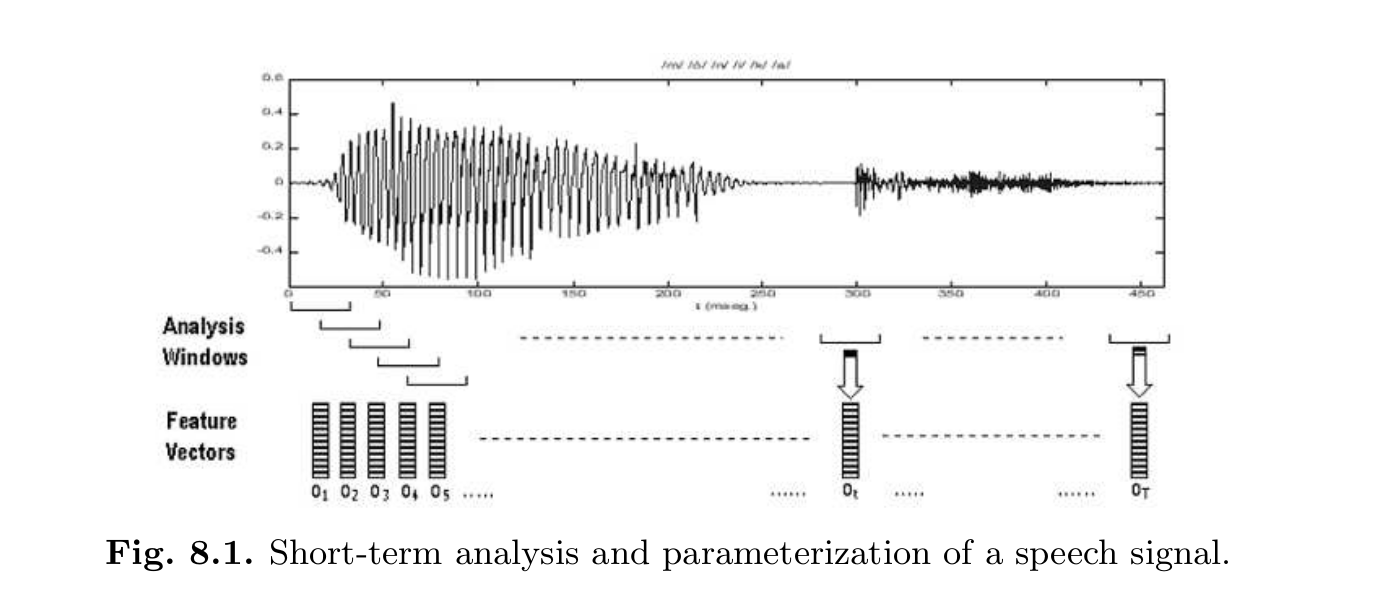
\includegraphics[width=1\linewidth]{images/figure_8_1.png}
		\caption{Phân tích theo từng đoạn ngắn và tham số hóa tín hiệu giọng nói}
		\label{fig:writing-thesis}
	\end{figure}

	\subsubsection{3.2 Tham số hóa (Parameterization)}
	\qquad Tín hiệu cửa sổ hamming/ hanning trong thời gian ngắn này có tất cả thông tin thời gian/ phổ mong muốn, mặc dù ở tốc độ bit cao (ví dụ: số hóa giọng nói điện thoại với tần số lấy mẫu 8 kHz trong một cửa sổ 32 ms. Có nghĩa là 256 mẫu x 16 bit / mẫu = 4096 bits = 512 bytes mỗi khung hình). 
	
	Phương pháp tham số hóa
	\begin{itemize}
		\item Linear Predictive Coding (LPC) 
		\item Mel-Frequency based Cepstral Coefficients (MFCC)
	\end{itemize}
	\textbf{Linear Predictive Coding (LPC)}
	\begin{figure}[H]
		\centering
		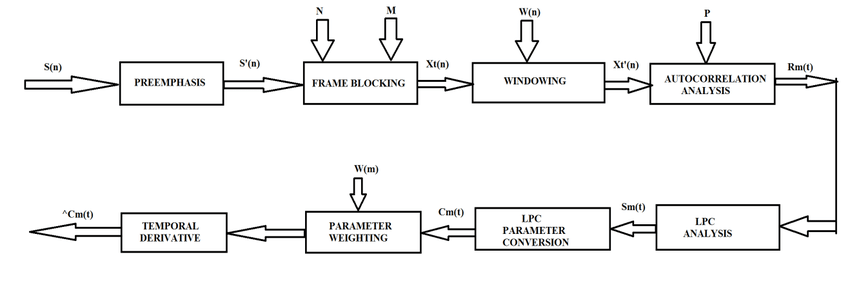
\includegraphics[width=1\linewidth]{images/Block-diagram-of-LPC-Linear-Predictive-Coding.png}
		\caption{Linear Predictive Coding (LPC) Diagram}
		\label{fig:writing-thesis}
	\end{figure}

	Linear Predictive Coding là một phương pháp sử dụng chủ yếu trong xử lý tín hiệu âm thanh và lời nói cho kết quả là đường bao phổ (đường cong đường bao của phổ biên độ - mô tả một điểm trong thời gian) của một số tín hiệu giọng nói dưới dạng nén, sử dụng thông tin của một mô hình dự đoán tuyến tính.

	\textbf{Mel-Frequency based Cepstral Coefficients (MFCC)}
	\begin{figure}[H]
		\centering
		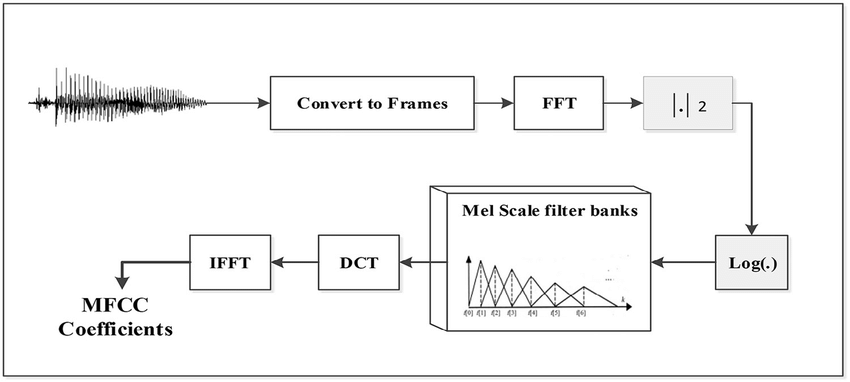
\includegraphics[width=1\linewidth]{images/Extraction-Mel-frequency-cepstral-coefficients-MFCC-from-the-audio-recording-signals.png}
		\caption{Linear Predictive Coding (LPC) Diagram}
		\label{fig:writing-thesis}
	\end{figure}

	Mel-Frequency based Cepstral Coefficients là một phương pháp để rút trích các đặc trưng (feature extraction) giọng nói thường được sử dụng trong các mô hình nhận dạng giọng nói tự động (Automatic Speech Recognition) hay phân lớp giọng nói (Speech Classification).
	\subsubsection{3.3 Phân tích ngữ âm và tách từ (Phonetic and word tokenization)}
	\qquad Mô hình Markov ẩn (HMM - Hidden Markov Models) là công cụ thành công nhất và được sử dụng rộng rãi (ngoại trừ một số kiến trúc ANN) để mã hóa ngữ âm, âm tiết và từ, nghĩa là dịch từ lời nói được lấy mẫu thành một căn chỉnh thời gian dãy các đơn vị ngôn ngữ.
	
	Huấn luyện HMM thường được thực hiện thông qua ước lượng Baum-Welch, trong khi giải mã và căn chỉnh thời gian thường được thực hiện thông qua giải mã Viterbi. Hiệu suất của các phổ HMM đó được cải thiện bằng cách sử dụng các mô hình ngôn ngữ, mô hình này áp đặt một số ràng buộc về ngôn ngữ hoặc ngữ pháp đối với sự kết hợp gần như vô hạn của tất cả các đơn vị có thể. Để cho phép tăng hiệu quả, việc lược bớt tìm kiếm chùm tia cũng là một cơ chế tổng quát để đẩy nhanh đáng kể quá trình nhận dạng mà không có hoặc ít suy giảm hiệu suất.
	
	\subsubsection{3.4 Phân tách ngữ điệu (Prosodic Tokenization)}
	\qquad Các đặc trưng ngữ điệu cơ sở như cao độ và năng lượng cũng có được ở mức frame. Năng lượng cửa sổ thu được rất dễ dàng thông qua định lý Parseval, ở dạng thời gian hoặc dạng phổ, và cao độ tức thời có thể được xác định bằng, ví dụ, phương pháp tự tương quan hoặc dựa trên phân rã cepstral, thường được làm mịn bằng một số lọc thời gian.
	
	 Các đặc điểm thuận âm quan trọng khác là những đặc điểm liên quan đến thời lượng của các đơn vị ngôn ngữ, tốc độ nói và tất cả những đặc điểm liên quan đến trọng âm. 
	 
	 Trong tất cả những trường hợp đó, cần phải phân đoạn chính xác, đánh dấu các vị trí âm tiết, đường nét năng lượng và cao độ để phát hiện các vị trí trọng âm và dấu chuyển cụm từ hoặc giọng nói. 
	 
	 Việc phân đoạn ngữ âm và âm tiết của lời nói là một vấn đề phức tạp còn lâu mới giải quyết được và mặc dù nó có thể hữu ích cho việc nhận dạng giọng nói, các hệ thống âm tiết không phải lúc nào cũng yêu cầu phân đoạn chi tiết như vậy.
	
	\subsection{4. Nhận dạng giọng nói phụ thuộc văn bản}
	
	\qquad Hệ thống nhận dạng giọng nói phụ thuộc văn bản, sử dụng nội dung từ vựng của giọng nói phát ra để nhận dạng giọng nói, ứng dụng chính của hệ thống này trong các hệ thống tương tác, nơi cần có sự hợp tác từ người dùng để xác thực danh tính của họ.
	
	Ví dụ điển hình của các ứng dụng này là xác thực bằng giọng nói qua điện thoại cho các hệ thống phản hồi giọng nói tương tác yêu cầu một số mức độ bảo mật như các ứng dụng ngân hàng hoặc đặt lại mật khẩu. 
	
	Tương tự như các phương thức sinh trắc học khác, việc sử dụng hệ thống nhận dạng giọng nói phụ thuộc vào văn bản yêu cầu giai đoạn đăng ký trong đó người dùng cung cấp một số mẫu để xây dựng mô hình người dùng và giai đoạn nhận dạng trong đó mẫu giọng nói mới được so khớp với mô hình người dùng.
		
	\subsubsection{4.1 Phân loại các hệ thống và kỹ thuật}
	\qquad Chúng ta có thể phân loại hệ thống nhận dạng người nói phụ thuộc vào văn bản theo quan điểm ứng dụng thành hai loại
	\begin{itemize}
		\item \textbf{Hệ thống văn bản tĩnh}:nội dung từ vựng trong ghi danh và các mẫu nhận dạng luôn giống nhau. Trong các \textbf{hệ thống văn bản động}, nội dung từ vựng trong mẫu nhận dạng là khác nhau trong mọi thử nghiệm truy cập với nội dung từ vựng của các mẫu đăng ký.
		\item \textbf{Hệ thống văn bản động}: tạo ra một lời nhắc mật khẩu được tạo ngẫu nhiên khác nhau mỗi khi người dùng được xác minh (hệ thống nhắc bằng văn bản), do đó hầu như không thể sử dụng bản ghi nên linh hoạt hơn và mạnh mẽ hơn trước các cuộc tấn công sử dụng bản ghi âm từ người dùng hoặc bắt chước sau khi nghe người nói thực sự nói đúng mật khẩu
	\end{itemize}
		
	Tuy nhiên, thông tin được sử dụng rộng rãi nhất là thông tin \textbf{phổ của tín hiệu tiếng nói}, được xác định bởi cấu hình vật lý và động lực của đường thanh quảng. Thông tin này thường được tóm tắt dưới dạng chuỗi thời gian của các vector MFCC, mỗi vector trong số đó đại diện cho một thời lượng nói từ 20-40 mili giây. Bằng cách này, vấn đề nhận dạng người nói phụ thuộc vào văn bản được giảm xuống thành vấn đề so sánh chuỗi các vector MFCC với mô hình của người dùng. 
	
	Có hai phương pháp đã được sử dụng rộng rãi: 
	\begin{itemize}
		\item \textbf{Phương pháp dựa trên khuôn mẫu}: bao gồm một số chuỗi vectơ tương ứng với lời nói đăng ký và việc nhận dạng được thực hiện bằng cách so sánh lời nói xác minh với lời nói đăng ký. So sánh này được thực hiện bằng cách sử dụng Dynamic Time Warping (DTW) như một cách hiệu quả để cải thiện sai lệch thời gian giữa các cách phát âm khác nhau.
		\item \textbf{Phương pháp thống kê}: Nổi bật nhất là \textbf{mô hình Markov ẩn (HMM)}, có xu hướng được sử dụng thường xuyên hơn các mô hình dựa trên khuôn mẫu. HMMs cung cấp tính linh hoạt hơn, cho phép chọn đơn vị tiếng nói từ đơn vị âm vị phụ đến từ và cho phép thiết kế hệ thống nhắc văn bản.
	\end{itemize}
	\subsubsection{4.2 Kho ngữ liệu}
	\begin{itemize}
		\item YOHO Speaker Verification
		\item MIT Mobile Device Speaker Verification Corpus
		\item BIOSEC Baseline Corpus
	\end{itemize}
	
	\subsubsection{4.3 Công trình điển hình}
	\textbf{Tên công trình} Text-dependent speaker recognition with HMM speaker adaptation and HMM reestimation 
	
	Hệ thống nhận dạng giọng nói phụ thuộc văn bản được thử nghiệm trên cơ sở dữ liệu chuẩn YOHO, hai hệ thống nhận dạng người nói phụ thuộc vào văn bản do các tác giả phát triển. Các hệ thống này mô phỏng một hệ thống được nhắc bằng văn bản dựa trên một tập hợp các HMM ngữ âm không phụ thuộc vào người nói và không phụ thuộc vào ngữ cảnh được đào tạo trên TIMIT.
	
	Giai đoạn đăng ký sử dụng một số câu của người nói để điều chỉnh HMM cho người đó. Ta so sánh hai cách thức thực hiện sự thích ứng này: Baum-Welch Reestimation và MLLR (maximum likelihood linear regression).
	Trong đó, Baum-Welch Reestimation là cách tiếp cận thông thường nhất nhưng yêu cầu sử dụng HMM rất đơn giản (chỉ một hoặc một vài Gaussian cho mỗi trạng thái) còn MLLR thì mới hơn và cho phép sử dụng các HMM phức tạp hơn.
	
	Một vấn đề quan trọng trong việc phát triển hệ thống nhận dạng giọng nói phụ thuộc văn bản là số lượng tài nguyên huấn luyện. YOHO chứa 4 phần với 24 câu nói mỗi phần, đây là một lượng tài nguyên đáng kể để huấn luyện một cách hiệu quả.
	
	\begin{figure}[H]
		\centering
		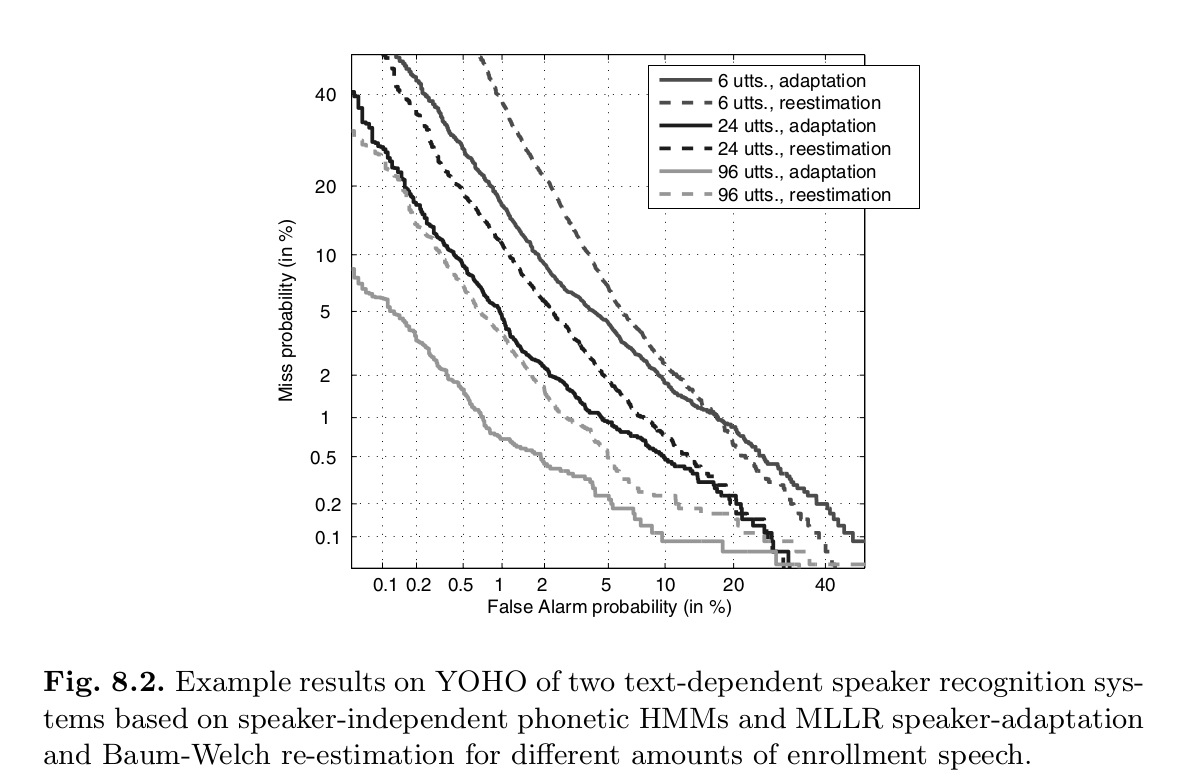
\includegraphics[width=1\linewidth]{images/figure_8_2.png}
		\caption{Linear Predictive Coding (LPC) Diagram}
		\label{fig:writing-thesis}
	\end{figure}
		
	\subsection{5. Nhận dạng giọng nói độc lập với văn bản}
	\qquad Hệ thống nhận dạng giọng nói độc lập với văn bản cố gắng giảm thiểu ảnh hưởng của nội dung từ vựng vốn được coi là không xác định đối với khả năng nhận dạng của giọng nói, điều này trái ngược với hệ thống nhận dạng giọng nói phụ thuộc văn bản, đương nhiên việc nghiên cứu và phát triển nó sẽ khó khăn hơn.
	
	\subsubsection{5.1 Short-term spectral systems - Hệ thống cửa sổ phổ âm}
	\qquad Khi phân tích phổ trong khoảng thời gian ngắn được sử dụng để mô hình các đặc trưng người nói, chúng ta đang mô hình hóa các “âm thanh” khác nhau mà một người có thế tạo ra, nhờ vào đường âm và các cơ quan cấu âm của họ. Khi con người cần nhiều âm thanh (hoặc các ký hiệu âm học khác nhau) để nói bằng bất kỳ ngôn ngữ chung nào, chúng ta rõ ràng đang đối mặt với một \textbf{không gian đa lớp gồm nhiều đặc trưng}.
	
	Kỹ thuật Lượng tử hóa Vector (\textbf{Vector Quantization techniques}) hiệu quả trong các bài toán đa lớp như vậy và đã được sử dụng để xác định người người, điển hình là một mô hình VQ cụ thể cho một người nói, tính toán khoảng cách từ bất kỳ câu nói nào đến bất kỳ mô hình nào dưới dạng tổng trong số của khoảng cách tối tiểu trên mỗi khung đến codevector gần của codebook. Việc sử dụng các giới hạn và các điểm trung tâm thay vì dùng mật độ xác suất làm hiệu suất của VQ kém hơn so với mô hình Markov ẩn với mật độ liên tục và liên thông hay còn gọi là Ergodic HMMs. 
	
	Tuy nhiên, yếu tố quan trọng trong \textbf{E-HMM} là tích số trạng thái với hàm Gaussian mỗi trạng thái, điều này loại bỏ triệt để ảnh hưởng của quá trình chuyển đổi trong mô hình liên thông. Sau đó, một hệ thống HMM với 5 trạng thái - 4 Gaussian cho mỗi trạng thái sẽ hoạt động tương tự như 4-trạng thái 5-Gaussian, 2-trạng thái 10-Gaussian, hoặc thậm chí là 1-trạng thái 20-Gaussian,  mà một cách hiểu tổng quát là GMM (\textbf{Gaussian Mixture Model}). Những one-state \textbf{E-HMMs} hoặc \textbf{GMMs} này có lợi thế lớn, tránh được cả ước lượng Baum-Welch cho việc huấn luyện, không cần sự liên kết giữa lời nói và trạng thái (tất cả lời nói đều được tinh chỉnh với cùng một trạng thái duy nhất) và dùng Viterbi decoding cho việc việc kiểm thử (không cần tinh chỉnh thời gian), giúp tăng tốc thời gian tính toán mà không ảnh hưởng đến hiệu suất.
	
	\textbf{GMM} là một kỹ thuật tổng hợp trong đó một hỗn hợp các hàm Gaussians Đa chiều cố gắng mô hình hóa phân phối thống kê chưa rõ của dữ liệu người nói. GMM trở thành một kỹ thuật hiện đại vào những năm 1990, cả khi \textbf{Maximum likehood} (Tối đa hóa kỳ vong \textbf{Expectation-Maximization}, EM) hoặc huấn luyện phân loại (\textbf{Maximum Mutual Information}, MMI) còn được dùng. Tuy nhiên, việc sử dụng MAP tương thích với hầu hết phương tiện từ một \textbf{Universal Background Model} (UBM) đã mang lại cho GMMs một lợi thế lớn so với các kỹ thuật khác, đặc biệt khi được sử dụng với các kỹ thuật chuẩn hóa như \textbf{Z-standar}d (chuẩn hóa điểm giả), \textbf{T-norm} (chuẩn hóa âm thanh), \textbf{H-norm} (chuẩn Z phụ thuộc vào thiết bị cầm tay), \textbf{HT-norm} (H + T-norm) hoặc \textbf{Feature Mapping} (xác định và chuẩn hóa kênh).
	
	\textbf{Discriminative techniques} - Kỹ thuật phân tách như \textbf{Artificial Neural Networks}, đã được sử dụng trong nhiều năm, nhưng hiệu suất của chúng chưa bao giờ đạt đến hiệu suất của \textbf{GMM}. Tuy nhiên, vào cuối những năm 90, \textbf{SVM - Support Vector Machine} được ví như một bộ phân loại hiệu năng cao được huấn luyện sẵn, mang lại cho \textbf{GMM} một đối thủ cạnh tranh vì hiệu suất gần như tương đương bằng việc sử dụng \textbf{SVM} trong không gian nhiều chiều hơn với các kernel tích hợp như GLDS (\textbf{Generalized Linear Discriminant Sequence Kernel})
	
	Gần đây, việc sử dụng \textbf{SuperVectors}, một kỹ thuật hỗn hợp \textbf{GMM-SVM} coi là công cụ của \textbf{GMM} cho mọi trường hợp (cả trong huấn luyện và kiểm tra) là các điểm trong không gian nhiều chiều (số chiều bằng với số hỗn hợp của \textbf{GMM} nhân với số chiều của vector được tham số hóa) bằng cách sử dụng \textbf{SVM} cho mỗi người nói để phân loại các cách phát âm chưa biết từ siêu phẳng giọng nói được huấn luyện sẵn.
	
	\subsubsection{5.2 Idiolectal systems - Hệ thống Idiolectal}
	\qquad Note: (Idiolectal = idio (personal, private) + (dia)lect)
	
	Hầu hết hệ thống nhận dạng người nói không phụ thuộc văn bản đều dựa vào đặc trưng phổ ngắn cho đến khi công trình của Doddington được công bố, nó mở ra một thế giới mới khả năng cải thiện các hệ thống nhận dạng người nói không phụ thuộc vào văn bản. 
	
	Doddington đã nhận ra và chứng minh rằng lời nói của những người nói khác nhau không chỉ khác nhau về âm học, mà còn về các đặc điểm khác như cách sử dụng từ. Đặc biệt, trong công việc của mình, ông đã lập mô hình cách sử dụng từ của từng người nói cụ thể bằng cách sử dụng \textbf{n-gram} mô hình hóa các chuỗi từ và xác suất của chúng và chứng minh rằng việc sử dụng các mô hình đó có thể cải thiện hiệu suất của hệ thống GMM âm thanh/ phổ cơ bản. Quan trọng hơn kết quả cụ thể này là thực tế là công trình này đã thúc đẩy nghiên cứu trong việc sử dụng các cấp độ thông tin cao hơn (idiolectal, phonotactic, prosodic, v.v.) để \textbf{nhận dạng giọng nói độc lập với văn bản}. 
	
	Các phần tiếp theo mô tả hai trong số những hệ thống thành công nhất khai thác mức độ thông tin cao hơn: hệ thống âm vị, cố gắng mô hình hóa các đặc điểm phát âm và hệ thống thuận âm, mô hình hóa các mẫu âm thanh chuyên biệt dành cho người nói.
	
	\subsubsection{5.3 Phonotactic systems - Hệ thống ngữ âm}
	\qquad Một hệ thống nhận dạng giọng nói phonotactic điển hình bao gồm hai khối chính:
	\begin{itemize}
		\item Bộ giải mã ngữ âm (the phonetic decoders), chuyển đổi lời nói thành một chuỗi các nhãn ngữ âm.
		\item Giai đoạn mô hình hóa ngôn ngữ thống kê n-gram, mô hình hóa tần số của ngữ âm và chuỗi ngữ âm cho mỗi người nói cụ thể.
	\end{itemize}

	\begin{figure}[H]
		\centering
		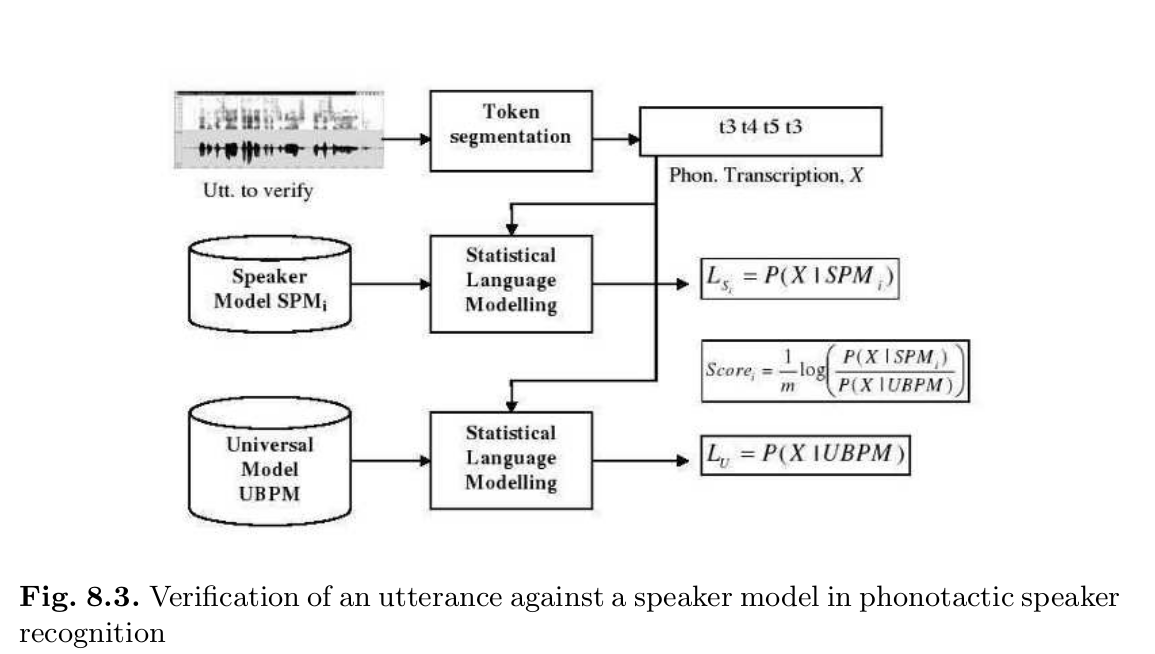
\includegraphics[width=1\linewidth]{images/figure_8_3.png}
		\caption{Quy trình của hệ thống ngữ âm}
		\label{fig:writing-thesis}
	\end{figure}
	
	\textbf{Bộ giải mã ngữ âm} – thường dựa trên \textbf{Mô hình Markov ẩn (HMMs)} - có thể được lấy từ trình nhận dạng giọng nói có sẵn hoặc được huấn luyện đặc biệt. Đối với mục đích nhận dạng người nói, việc có bộ giải mã ngữ âm không quan trọng và thậm chí không quan trọng lắm phải có bộ giải mã ngữ âm trong ngôn ngữ của người nói để được nhận dạng. Thực tế có phần đáng ngạc nhiên này đã được phân tích cho thấy rằng các lỗi ngữ âm phụ thuộc vào giọng nói do bộ giải mã tạo ra dường như là của giọng nói cụ thể và do đó thông tin hữu ích cho việc nhận dạng giọng nói miễn là các lỗi này phù hợp với từng giọng nói cụ thể.
	
	Sau khi có bộ giải mã ngữ âm, bản giải mã ngữ âm của nhiều câu từ nhiều giọng nói khác nhau có thể được sử dụng để huấn luyện \textbf{Mô hình Universal Background Phone} ($UBPM$) đại diện cho tất cả những giọng nói có thể có. Các \textbf{Mô hình Ngữ âm Giọng nói} ($SPM_i$ - \textbf{Speaker Phone Models}) được huấn luyện bằng cách sử dụng một số bộ giải mã ngữ âm của từng người nói cụ thể. Vì giọng nói có sẵn để huấn nói một mô hình giọng nói thường bị hạn chế, các mô hình giọng nói được nội suy với $UBPM$ để tăng tính mạnh mẽ trong ước tính tham số. 
	
	Sau khi các mô hình ngôn ngữ thống kê được huấn luyện, quy trình để xác minh cách phát âm một tập test so với mô hình giọng nói $SPM_i$ gồm các bước:
	\begin{itemize}
		\item Bước 01: Tạo ra giải mã ngữ âm của nó, $X$, giống như cách giải mã được sử dụng để huấn luyện $SPM_{i}$ và $UBPM$
		\item Bước 02: Giải mã ngữ âm của câu thử, $X$ và các mô hình thống kê ($SPM_{i}$, UBPM) được sử dụng để tính toán khả năng giải mã ngữ âm, $X$, dựa trên mô hình giọng nói $SPM_{i}$ và mô hình nền $UBPM$. 
	\end{itemize}
		
	\textbf{Điểm nhận dạng là logarith tỷ lệ của cả hai khả năng xảy ra}. Quá trình này, thường được mô tả là Nhận dạng ngữ âm, sau đó là Mô hình hóa ngôn ngữ ($PRLM$) có thể được lặp lại cho các bộ giải mã ngữ âm khác nhau (ví dụ: các ngôn ngữ hoặc độ phức tạp khác nhau) và các điểm nhận dạng khác nhau chỉ được thêm vào hoặc hợp nhất để có hiệu suất tốt hơn, mang lại một phương pháp được gọi là $PRLM$ hoặc $PPRLM$ song song.
	
	Để cải thiện hiệu năng người ta sử dụng toàn bộ mạng lưới nhận dạng ngữ âm, nó là một đồ thị không chu trình có hướng chứa các giả thuyết có khả năng xảy ra nhất cùng với các xác suất của chúng. Có nhiều thông tin có nghĩa cho phép ước tính \textbf{n-gam} tốt hơn trên các tài nguyên giọng nói hạn chế. Ngoài ra, hiệu năng còn có thể cải thiện bằng việc sử dụng \textbf{SVM} để phân lớp toàn bộ n-gam được huấn luyện với giả thuyết tốt nhất.
	
	\textbf{Tóm tắt các bước hoạt động của mô hình}
	\begin{itemize}
		\item Bước 1: Đầu vào là giọng nói cần xác minh
		\item Bước 2 - Token segmentation: Tách thành các đoạn t3, t4, t5, t3
		\item Bước 3: Mô hình hóa ngôn ngữ thống kê n-gram
		\begin{itemize}
			\item Huấn luyện mô hình Universal Background Phone (UBPM) $L_{U} = P(X|UBPM)$
			\item Huấn luyện mô hình Speaker Phone Models ($SPM_{i}$): $L_{S_{i}} = P(X | SPM_{i})$
		\end{itemize}
		\item Bước 4: Tính recognition score: $Score_{i} = \frac{1}{m}log\left(\frac{P(X | SPM_{i})}{P(X|UBPM)}\right)$
	\end{itemize}

	\begin{figure}[H]
		\centering
		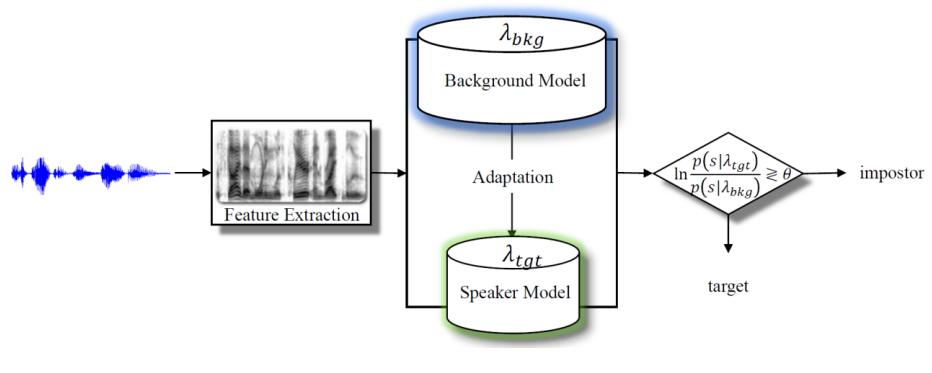
\includegraphics[width=1\linewidth]{images/diagram.png}
		\caption{Quy trình của hệ thống ngữ âm}
		\label{fig:writing-thesis}
	\end{figure}
	
	\subsubsection{5.4 Prosodic systems - Hệ thống ngữ điệu}
	\qquad Một trong những hệ thống ngữ điệu tiên phong và thành công nhất trong việc nhận dạng giọng nói không phụ thuộc vào văn bản là công trình của Adami. Hệ thống bao gồm hai khối xây dựng chính: 
	\begin{itemize}
		\item Phân tách ngữ điệu, phân tích ưu điểm và biểu thị nó dưới dạng một chuỗi các nhãn hoặc token
		\item Mô hình hóa ngôn ngữ thống kê n-gram, mô hình hóa tần số của các tokens và trình tự của từng giọng nói cụ thể
	\end{itemize}
	 
	 Một số khả năng khác để mô hình hóa thông tin ngữ điệu cũng đã được chứng minh là khá thành công là việc sử dụng Non-uniform Extraction Region Features (NERFs) được phân định bằng khoảng dừng đủ dài hoặc NERF được xác định bởi cấu trúc âm tiết của câu (SNERFs).
	
	Các tác giả đã triển khai một hệ thống ngữ điệu dựa trên công trình của Adami, trong đó khối thứ hai giống hệt nhau để nhận dạng ngữ âm và âm sắc chỉ với những điều chỉnh nhỏ để cải thiện hiệu suất. Quá trình tokenization bao gồm hai giai đoạn:
	\begin{itemize}
		\item Giai đoạn một, đối với mỗi đoạn giọng nói của đoạn thoại, quỹ đạo thời gian của các đặc điểm thuận (tần số cơ bản - hoặc cao độ- và năng lượng) được rút trích
		\item Giai đoạn hai, cả hai đường bao đều được phân đoạn và dán nhãn bằng định lượng trung bình độ dốc.
	\end{itemize}

	\begin{figure}[H]
		\centering
		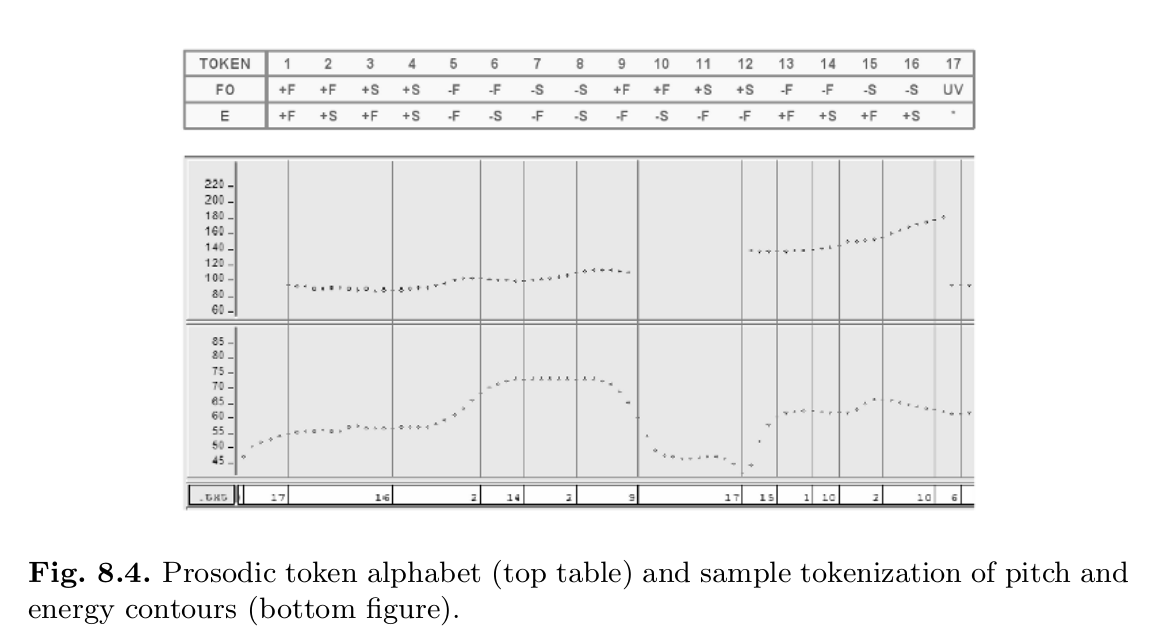
\includegraphics[width=1\linewidth]{images/figure_8_4.png}
		\caption{Token ngữ điệu alphabet}
		\label{fig:writing-thesis}
	\end{figure}

	Hình trên là một bảng chứa 17 token ngữ điệu. Một token đại diện cho các phân đoạn vô thanh, trong khi 16 token được sử dụng để đại diện cho các phân đoạn hữu thanh tùy thuộc vào độ dốc (phát nhanh, tăng chậm, giảm nhanh, giảm chậm) của năng lượng và cao độ.
	
	\subsubsection{5.5 Kho ngữ liệu và benchmarks}
	\begin{itemize}
		\item Vào năm 1996, NIST bắt đầu Đánh giá Nhận dạng Giọng nói -Speaker Recognition Evaluations hàng năm, đây chắc chắn là động lực của những tiến bộ đáng kể.
		\item Các hội thảo sau đánh giá đã cho phép người tham gia chia sẻ kinh nghiệm, cải tiến, thất bại, v.v. của họ trong một môi trường hợp tác cao. Vai trò của LDC (Linguistic Data Consortium) cung cấp tài liệu nói mới đầy thách thức cũng rất đáng chú ý, vì nhu cầu liên tục tăng lên (cả về lượng lời nói và yêu cầu ghi âm)
		\item Các bộ đánh giá trước đây (phát triển, huấn luyện và kiểm tra âm thanh và chìa khóa giải pháp) có sẵn thông qua LDC - Linguistic Data Consortium để các nhà nghiên cứu mới đánh giá hệ thống của họ mà không có áp lực cạnh tranh
	\end{itemize}
	
	\subsubsection{5.6 Công trình điển hình}
	\textbf{Tên công trình}: The ATVS multilevel text-independent system
	\begin{figure}[H]
		\centering
		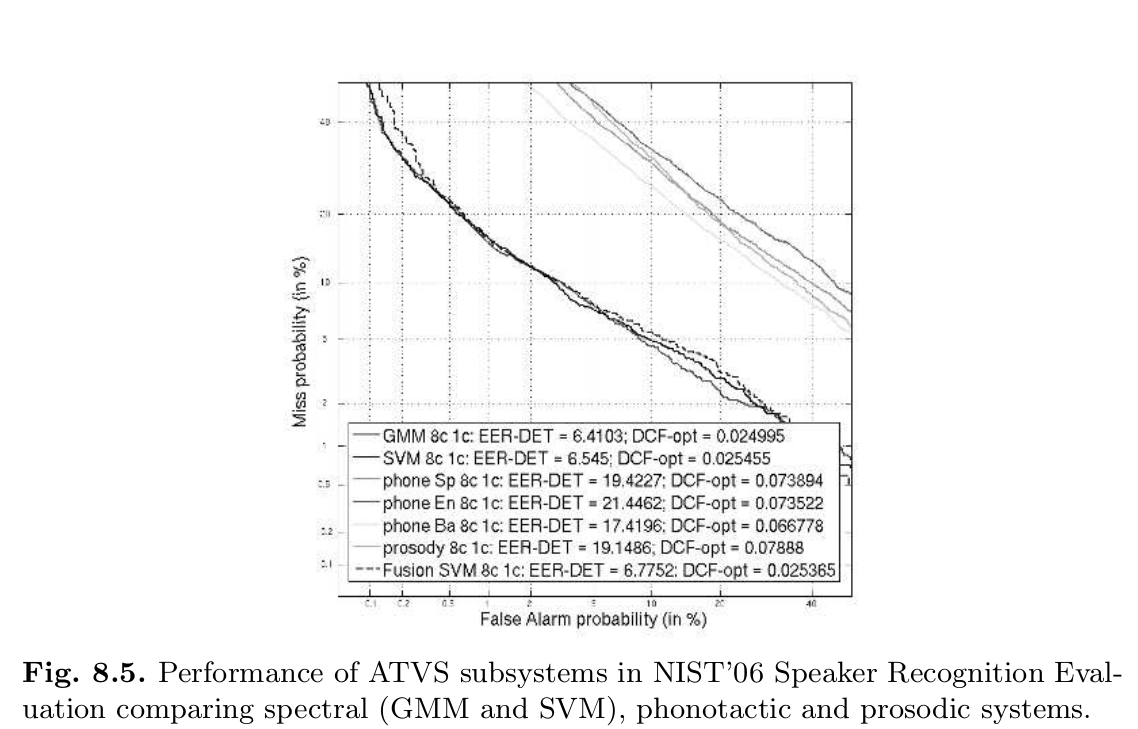
\includegraphics[width=1\linewidth]{images/figure_8_5.png}
		\caption{Linear Predictive Coding (LPC) Diagram}
		\label{fig:writing-thesis}
	\end{figure}

	Kết quả tại NIST SRE06 trong nhiệm vụ 8c1c (8 conversation for training và 1 conversation for testing), để xem hiệu suất của các hệ thống con khác nhau trên cùng một bài tập. Sự khác biệt chính của hệ thống ATVS năm 2006 so với hệ thống 2005 là việc sử dụng Ánh xạ đặc trưng trong cả GMM và SVM, việc sử dụng mở rộng đa thức bậc 3 (thay vì bậc 2) trong nhân GLDS và việc sử dụng của một PRLM được huấn luyện với SpeechDat
	
	\begin{figure}[H]
		\centering
		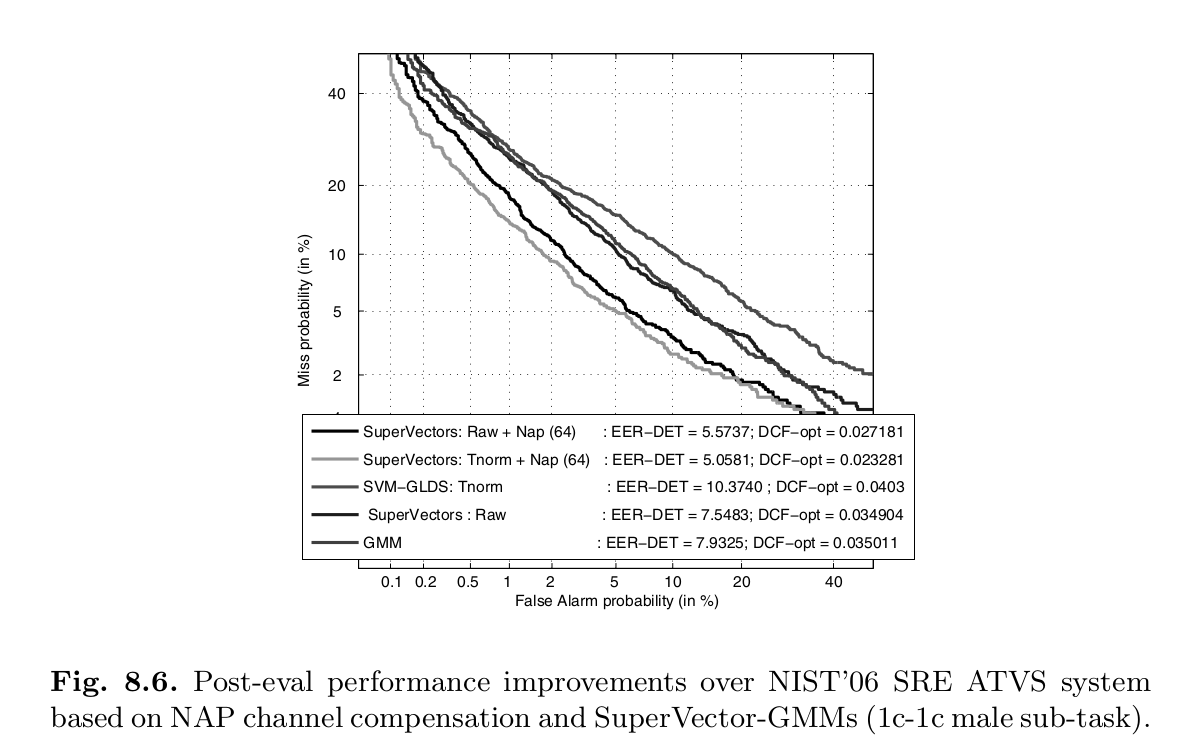
\includegraphics[width=1\linewidth]{images/figure_8_6.png}
		\caption{Linear Predictive Coding (LPC) Diagram}
		\label{fig:writing-thesis}
	\end{figure}

	\section{D.2 Các phương pháp SOTA - State of The Art gần đây về Voice Biometrics}
	\subsection{D.2.1 Giới thiệu}
	Những phương pháp đã tìm hiểu từ sách Handbook of Biometrics: Voice Biometrics đã cho chúng ta cái nhìn tổng quan về lĩnh vực Nhận dạng giọng nói và những phương pháp truyền thống (tạm gọi là thời kỳ trước Deep Learning) cùng với những thông tin các công trình nghiên cứu nổi bật. Tuy nhiên, gần đây với sự phát triển trong lý thuyết Học Máy cùng với những thành công đầy hy vọng của Học Sâu (Deep Learning) thì lĩnh vực Nhận dạng Giọng nói đã và đang tiếp tục phát triển.
	
	\subsection{D.2.2 Động lực nghiên cứu}
	Hai tác vụ lớn trong lĩnh vực Nhận dạng giọng nói (Speaker Recognition) là định danh giọng nói (Speaker Identification) và xác minh giọng nói (Speaker Verification) vẫn đã và đang phát triển, song song với sự phát triển của công nghệ.
	
	Lĩnh vực nghiên cứu này có nhiều ứng dụng trong thực tế, áp dụng vào nhiều lĩnh vực khác như bảo mật, pháp y, xác thực sinh trắc học, nhận dạng người nói và phân cực người nói. Nhiều phương pháp SOTA (State of the Art) được đưa nhằm giải quyết bài toán nhận dạng giọng nói ngày càng tốt hơn, đặc biệt là sử dụng kỹ thuật Deep Learning. 
	
	Với mục đích mở rộng kiến thức về nó, trong phần trình bày này, nhóm xin phép trình bày những gì tìm hiểu được về những phương pháp nhận dạng giọng nói nổi bật gần đây (khoảng 2014 - đến nay) 
	
	\subsection{D.2.3 Phát biểu bài toán}
	\textbf{Tác vụ:} Định danh người nói
	\begin{itemize}
		\item Đầu vào (Input): Dữ liệu âm thanh giọng nói
		\item Đầu ra (Output): Danh tính của người nói
	\end{itemize}
	\textbf{Tác vụ:} Xác nhận người nói
	\begin{itemize}
		\item Đầu vào (Input): Dữ liệu âm thanh giọng nói
		\item Đầu ra (Output): Đồng ý/ Từ chối
	\end{itemize}

	\subsection{D.2.4 Một số kho ngữ liệu}
	\qquad Cũng giống như các lĩnh vực khác của Học Máy, câu hỏi quan trọng ngay từ ban đầu là dữ liệu. Trong phần này, nhóm giới thiệu một số cơ sở dữ liệu phục vụ cho việc huấn luyện các mô hình, cho các tác vụ như speaker identification, speaker verification, speaker recognition.\newline
	\textbf{Kho ngữ liệu TIMIT (Garofolo et al., 1993)}
	\begin{itemize}
		\item Tên đầy đủ: TIMIT Acoustic-Phonetic Continuous Speech Corpus
		\item Tác giả/ Nhóm tác giả: 	John S. Garofolo, Lori F. Lamel, William M. Fisher, Jonathan G. Fiscus, David S. Pallett, Nancy L. Dahlgren, Victor Zue
		\item Năm: 1993
		\item Ngôn ngữ: Tiếng Anh
		\item Mô tả sơ lược: TIMIT chứa các bản ghi âm băng thông rộng của 630 người nói tám phương ngữ chính của tiếng Anh Mỹ, mỗi người đọc mười câu giàu ngữ âm. Kho tài liệu TIMIT bao gồm các phiên âm từ ngữ, ngữ âm và từ ngữ được căn chỉnh theo thời gian cũng như tệp dạng sóng giọng nói 16 bit, 16kHz cho mỗi câu nói
	\end{itemize}	
	\textbf{Kho ngữ liệu WSJ (Marcus et. al, 1993)}
	\begin{itemize}
		\item Tên đầy đủ: CSR-I (WSJ0) Complete
		\item Tác giả/ Nhóm tác giả: John S. Garofolo, David Graff, Doug Paul, David Pallett
		\item Năm: 1993
		\item Ngôn ngữ: Tiếng Anh
		\item Mô tả sơ lược: 
	\end{itemize}	
	\textbf{Kho ngữ liệu RSR2015 (Larcher et al., 2012)}
	\begin{itemize}
		\item Tên đầy đủ: The RSR2015: Database for Text-Dependent Speaker Verification using Multiple Pass-Phrases
		\item Tác giả/ Nhóm tác giả: Anthony Larcher, Kong Aik Lee, Bin Ma, Haizhou Li
		\item Hội nghị: Annual Conference of the International Speech
		Communication association (Interspeech), tại Portland, United States, năm 2012
		\item Mô tả sơ lược: Cơ sở dữ liệu RSR2015 chứa các bản ghi âm từ 300 người, 143 nữ và 157 diễn giả nam. Những người tham gia được chọn để trở thành đại diện cho sự phân bố dân tộc của người Singapore. Các diễn giả được chọn từ 17 đến 42 tuổi. Mỗi người trong số những người tham gia ghi lại chín phiên bằng cách sử dụng ba thiết bị di động. Mỗi phiên bao gồm ba mươi câu ngắn.
	\end{itemize}
	\textbf{Kho ngữ liệu Librispeech (Panayotov et.al, 2015)}
	\begin{itemize}
		\item Tên đầy đủ: LibriSpeech ASR corpus
		\item Bài báo: LibriSpeech: an ASR corpus based on public domain audio books
		\item Tác giả/ Nhóm tác giả: Vassil Panayotov, Guoguo Chen, Daniel Povey and Sanjeev Khudanpur
		\item Được công bố tại hội nghị The international Conference on Acoustics, Speech, \& Signal Processing (ICASSP), 2015
		\item Mô tả sơ lược: Kho ngữ liệu có kích thước khoảng 1000 giờ nói tiếng Anh với tần số 16kHz
	\end{itemize}	
	\textbf{Kho ngữ liệu VCTK (Veaux et al., 2017)}
	\begin{itemize}
		\item Tên đầy đủ: SUPERSEDED - CSTR VCTK Corpus: English Multi-speaker Corpus for CSTR Voice Cloning Toolkit
		\item Tác giả/ Nhóm tác giả: Veaux Christophe, Yamagishi Junichi, MacDonald Kirsten
		\item Nhà xuất bản: University of Edinburgh. The Centre for Speech Technology Research (CSTR)
		\item Mô tả sơ lược:
	\end{itemize}
	\textbf{Kho ngữ liệu VoxCeleb (Nagrani et. al, 2017)}
	\begin{itemize}
		\item Tên đầy đủ: VoxCeleb: a large-scale speaker identification dataset
		\item Tác giả/ Nhóm tác giả: Arsha Nagrani, Joon Son Chung, Andrew Zisserman (Visual Geometry Group, Department of Engineering Science, University of Oxford, UK)
		\item Mô tả sơ lược: kho ngữ liệu chứa hơn 100.000 câu nói cho 1.251 người nổi tiếng, được trích xuất từ các video tải lên YouTube. Bộ dữ liệu cân bằng về giới tính, với 55\% người nói là nam giới. Các diễn giả trải dài một loạt các sắc tộc, giọng, nghề nghiệp và độ tuổi khác nhau. Quốc tịch và giới tính của mỗi người nói (lấy từ Wikipedia) cũng được cung cấp.
	\end{itemize}
	\textbf{Kho ngữ liệu VoxCeleb2 (Chung et. al, 2018)}
	\begin{itemize}
		\item Tên đầy đủ: VoxCeleb2: Deep Speaker Recognition  
		\item Tác giả/ Nhóm tác giả: J. S. Chung*, A. Nagrani*, A. Zisserman
		\item Hội nghị: INTERSPEECH, 2018.  
		\item Mô tả sơ lược: Là kho ngữ liệu giọng nói lớn nhất hiện tại, VoxCeleb2 chứa hơn 1 triệu câu nói cho 6.112 người nổi tiếng, được trích xuất từ các video tải lên YouTube. Tập hợp phát triển của VoxCeleb2 không có sự trùng lặp với các đặc điểm nhận dạng trong tập dữ liệu VoxCeleb1 hoặc SITW.
	\end{itemize}
	\subsection{D.2.5 Kiểm định mô hình nhận dạng giọng nói}
	Trong xác minh người nói, để đưa ra quyết định người ta đề xuất kiểm tra bằng cách sử dụng likelihood-ratio test.

	\subsection{D.2.5 Các độ đo trong nhận dạng giọng nói}
	
	Trong nhận dạng giọng nói (đặc biệt là tác vụ xác minh), có hai loại độ đo tính tương tự thường được sử dụng để tính toán xác suất nếu một quan sát thử nghiệm có phải từ người nói đích hay không. Hầu hết tất cả các phương pháp tiếp cận bằng Deep Learning mới đều sử dụng các độ đo này (trong các sơ đồ xác minh người nói): khoảng cách cosin của những vector (Cosine Distance) và PLDA (Phân tích phân tách tuyến tính theo xác suất - probabilistic linear discriminant analysis).
	
	\textbf{Khoảng cách Cosine - Cosine Distance}
	Một trong những độ đo đơn giản mà lại hiệu quả đó là khoảng cách Cosine, việc xác minh người nói được xác nhận thông qua góc giữa hai vectors, nếu góc càng bé, nghĩa là hai giọng nói càng gần nhau và ngược lại, khi góc giữa chúng càng lớn, nghĩa là hai giọng nói càng xa nhau, khác nhau.
	\begin{align*}
		CDS(w_{\text{target}}, w_{\text{test}}) = \frac{w_{\text{target}}.w_{\text{test}}}{||w_{\text{target}}||.||w_{\text{test}}||}
	\end{align*}
	
	\textbf{Phân tích phân tách tuyến tính theo xác suất - probabilistic linear discriminant analysis}
	Cho tập hợp i-vectors d chiều có độ dài chuẩn đã được chuẩn hóa 
	$$X = \{x_{ij}; i = \overline{1..N}, j = \overline{1..N}\}$$ thu được từ N người nói huấn luyện (mỗi người nói có $H_{i}$ i-vectors), i-vectors có thể được viết dưới dạng:
	$$x_{ij} = \mu + Wz_{i} + \epsilon_{ij}$$
	Với $x_{ij} \in \mathbb{R}^{D}, W \in \mathbb{R}^{ \times M}, z_{i} \in \mathbb{R}^{M}, \epsilon_{ij} \in \mathbb{R}^{D}$
	
	Tập $Z=\{z_{j}, i = \overline{1..N}\}$ là các ẩn số
	
	$W$ là ma trận kích thước $D \times M$ gọi là ma trận tải dữ kiện
	
	$\mu$ là trung bình tập $X$
	
	$z_{i}$ gọi là dữ kiện người nói
	
	$\epsilon_{ij}$ nhiễu với phân bố Gaussian trung bình 0 và hiệp phương sai $\Sigma$
	
	Cho một i-vector kiểm tra $x_t$ và một người nói cần được kiểm tra có i-vector $x_s$, điểm LR được tính toán như sau :
	$$S_{LR}(x_t, x_s) = \frac{P(x_s, x_t|\text{same speaker})}{P(x_s, x_t|\text{different speaker})}$$
	$$\Leftrightarrow S_{LR}(x_t, x_s) = 
	\frac{N([x_s^Tx_t^T]|[\mu^T\mu^T], \hat{W}\hat{W}^T + \hat{\Sigma})}{N([x_s^Tx_t^T]|[\mu^T\mu^T],diag\{WW^T+\Sigma, WW^T+\Sigma\})}$$
	Trong đó:
	\begin{itemize}
		\item $\hat{W} = [W^TW^T]^T$
		\item $\hat{\Sigma}=diag\{\Sigma,\Sigma\}$
	\end{itemize}
	Sử dụng công thức chuẩn cho nghịch đảo của ma trận khối trích trong Petersen, K. B., Pedersen, M. S. (2008). The matrix cookbook.
	Technical University of Denmark, 7(15), 510, trích trong bài báo Ioffe, S. (2006). Probabilistic linear discriminant analysis. In:
	European Conference on Computer Vision. Springer, Berlin,
	Heidelberg, pp. 531-542. Thu được công thức: 
	$$S_{LR}(x_s, x_t) = const + x_s^TQx_s + x_t^TQx_x^T + 2x_s^TPx_t$$
	Trong đó: 
	\begin{itemize}
		\item $P = \Lambda ^{-1}\Gamma(\Lambda - \Gamma\Lambda^{-1}\Gamma)^{-1};\Lambda=WW^T+\Sigma$
		\item $Q = \Lambda ^{-1}(\Lambda - \Gamma\Lambda^{-1}\Gamma)^{-1};\Gamma=WW^T$
	\end{itemize}
	
	
	\subsection{D.2.5 Học Sâu trong tác vụ rút trích đặc trưng giọng nói}
	\subsubsection{D.2.5.1 Về d-vectors}
	\begin{figure}[H]
		\centering
		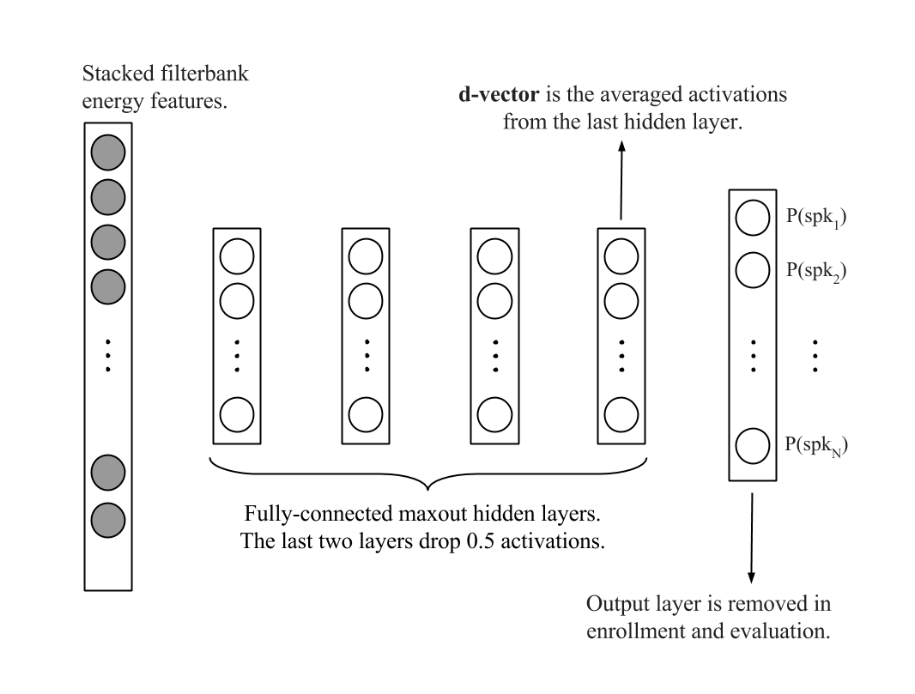
\includegraphics[width=0.75\linewidth]{images/d-vectors.png}
		\caption{DNN model for speaker verification - Deep Neural Networks for small foot-print text-dependent speaker verification - 2014}
		\label{fig:writing-thesis}
	\end{figure}
	\qquad Được giới thiệu trong bài báo "Deep neural networks for small footprint text-dependent speaker verification" \textbf{d-vectors} trở thành tiền đề cho hàng loạt các thành công sau này của lĩnh vực Nhận dạng giọng nói sử dụng Deep Learning.
	
	\textbf{Giới thiệu chung về bài báo:}
	\begin{itemize}
		\item Bài báo: Deep neural networks for small footprint text-dependent speaker verification (Một bước nhỏ trong dùng mạng học sâu cho tác vụ xác minh người nói)
		\item Nhóm tác giả: Ehsan Variani (Johns Hopkins Univ., Baltimore, MD, USA), Xin Lei (Google Inc., USA), Erik McDermott (Google Inc., USA), Ignacio Lopez Moreno (Google Inc, Mountain View, CA, US), Javier Gonzalez-Dominguez (Google Inc., USA)
		\item Được publish tại hội nghị 2014 IEEE International Conference on Acoustics, Speech and Signal Processing (ICASSP), diễn ra tại Florence, Italy, vào năm 2014
		\item Từ khóa: Deep Neural Networks, Speaker Verification
	\end{itemize}

	Trong bài báo này, nhóm tác giả trình bày việc sử dụng Deep Neural Networks trong tác vụ xác minh người nói (Speaker Verification) để rút trích đặc trưng giọng nói và kích hoạt đặc trưng nằm lớp ẩn cuối cùng của mạng học - gọi là d-vectors (Deep Vectors)
	
	Trong giai đoạn đăng ký (Speaker Enrollment), mô hình DNN được huấn luyện sẵn được sử dụng để rút trích đặc trưng giọng nói của người nói ở lớp cuối cùng. Sau đó tính toán giá trị trung bình của những đặc trưng này, để cho ra d-vector của người nói

	Trong giai đoạn đánh giá (Evaluation Stage), một giọng nói cần được xác minh khi vào mô hình sẽ được tính toán để cho ra một d-vector. Sau đó, dùng d-vector này so sánh với những d-vector trong quá trình đăng ký để đưa ra quyết định giọng nói của người nói này có phải là đúng với danh tính đưa ra không. Việc so sánh ở đây dùng độ đo cosine giữa hai vectors, việc đưa ra quyết định xác nhận sẽ dựa vào một ngưỡng (threshold)
	
	Do điều kiện tài nguyên hạn chế, nhóm tác giả dùng maxout DNN sử dụng chiến lược dropout, chiến lược này giúp tránh việc over-fitting khi huấn luyện mô hình học trên tập dữ liệu huấn luyện nhỏ
	
	Mô hình maxout DNN với 4 tầng ẩn (hidden layers) với 256 node cho mỗi tầng, không dùng DistBelief framework, kích thước pool mỗi tần là 2. Hai tầng đầu tiên không sử dụng dropout, hai tầng cuối sẽ drop 50\% activations
	
	Hàm Activation ở mỗi đơn vị neuron là một hàm phi tuyến, learning rate 0.001 với phân rã cấp số nhân (0.1 cho mỗi 5 triệu bước).
	
	Đầu vào DNN được tạo ra bằng cách xếp chồng các đặc trưng được rút trích từ một khung bằng tập các bộ lọc 40 chiều. Số chiều của vector target sẽ tương ứng với số người nói tập huấn luyện, ở đây nhóm tác giả đưa ra là 496. Cuối cùng, mô hình DNN sẽ chứa khoảng 600k tham số, tương dương với một hệ thống i-vectors nhỏ nhất!
	
	\textbf{Phương pháp thực nghiệm}
	Tập dữ liệu chứa 646 người nói, nói cùng một câu "ok google" nhiều lần trong nhiều cách khác nhau.
	
	Sau đó, 496 người nói sẽ được chọn một cách ngẫu nhiên dùng làm tập huấn luyện, 150 người nói còn lại sẽ được dùng để đăng ký và đánh giá
	
	Trong quá trình huấn luyện, số lần nói của mỗi người nói sẽ thay đổi từ 60 đến 130
	
	Trong quá trình đăng ký người nói, 20 câu nói đầu tiên sẽ dành cho việc ghi danh tính và còn lại sẽ dùng cho việc đánh giá
		
	\textbf{Các kết quả}
	
	So sánh kết quả EER của hệ thống i-vectors so với các hệ thống khác như Gaussians, LDA cho thấy sự vượt trội hơn hẳn cho hệ thống i-vectors
	\begin{figure}[H]
		\centering
		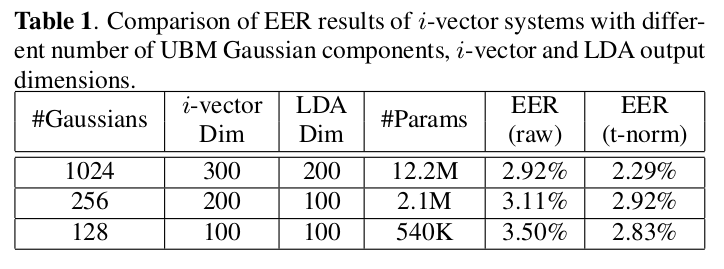
\includegraphics[width=0.75\linewidth]{images/d-vectors-result-table-01.png}
		\caption{- Deep Neural Networks for small foot-print text-dependent speaker verification - 2014}
		\label{fig:writing-thesis}
	\end{figure}
	Các kết quả EER của hệ thống xác nhận i-vectors và d-vectors  với số câu nói đăng ký khác nhau. Chúng ta có thể thấy độ lỗi giảm dần khi cho số lượng câu nói tăng lên. Tuy nhiên, hệ thống d-vectors không có nhiều sự vượt trội hơn hẳn so với i-vectors.
	\begin{figure}[H]
		\centering
		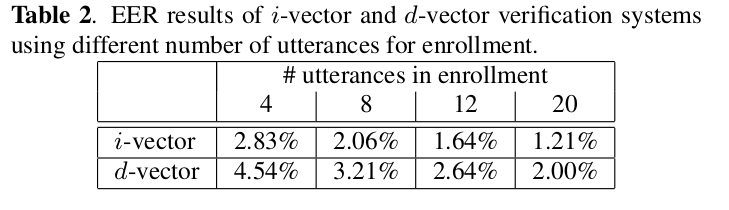
\includegraphics[width=0.75\linewidth]{images/d-vectors-result-table-02.png}
		\caption{- Deep Neural Networks for small foot-print text-dependent speaker verification - 2014}
		\label{fig:writing-thesis}
	\end{figure}

	Đồ thị bên dưới thể hiện đường cong DET giữa i-vector và d-vector sử dụng raw và t-norm.Ta có thể thấy, xác suất đồng ý sai của d-vector khá tốt so với i-vectors trong điều kiện dữ liệu sạch và nhiễu tương đối, tuy nhiên chưa có nhiều sự vượt trội đáng kể.
	\begin{figure}[H]
		\centering
		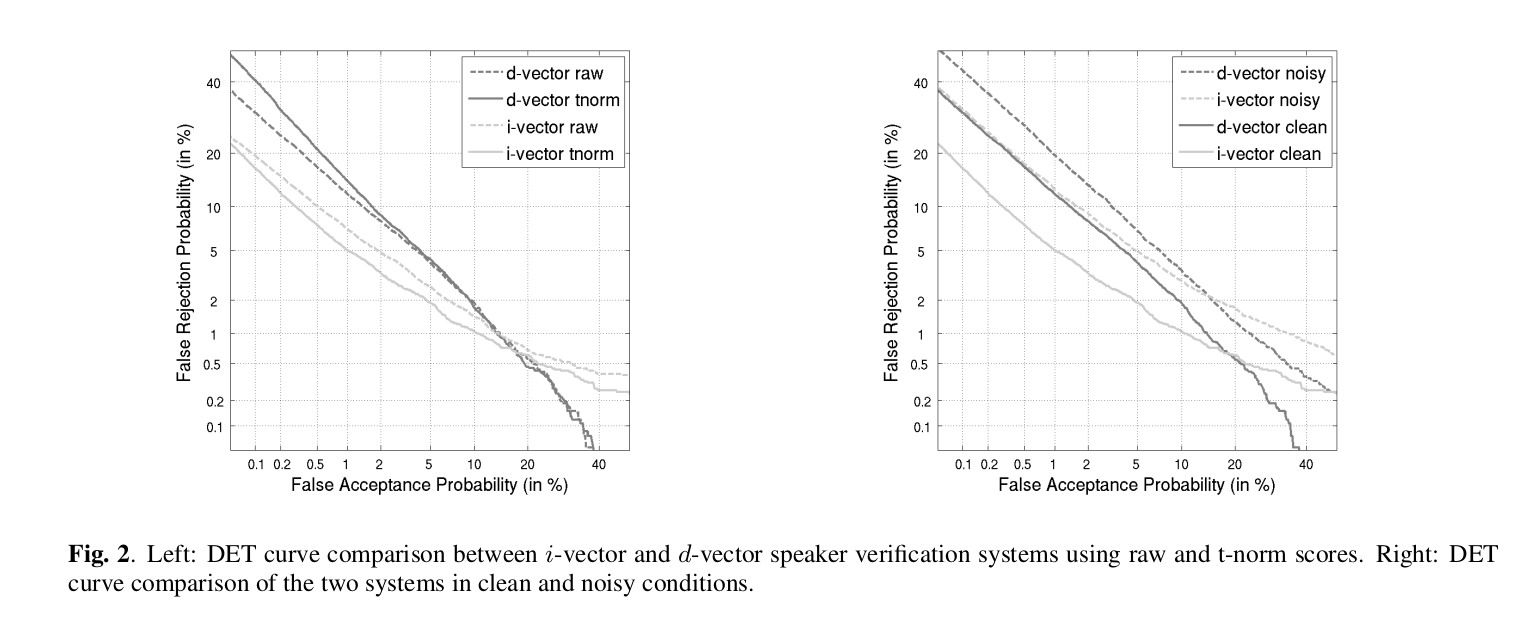
\includegraphics[width=0.85\linewidth]{images/i-vectors-d-vectors-det-compare.png}
		\caption{- Deep Neural Networks for small foot-print text-dependent speaker verification - 2014}
		\label{fig:writing-thesis}
	\end{figure}

	Đồ thị bên dưới thể hiện đường cong DET giữa i-vector và d-vector sử dụng raw và t-norm.Ta có thể thấy, xác suất từ chối sai của d-vector khá tốt so với i-vectors trong điều kiện dữ liệu sạch và nhiễu tương đối, tuy nhiên chưa có nhiều sự vượt trội đáng kể.
	\begin{figure}[H]
		\centering
		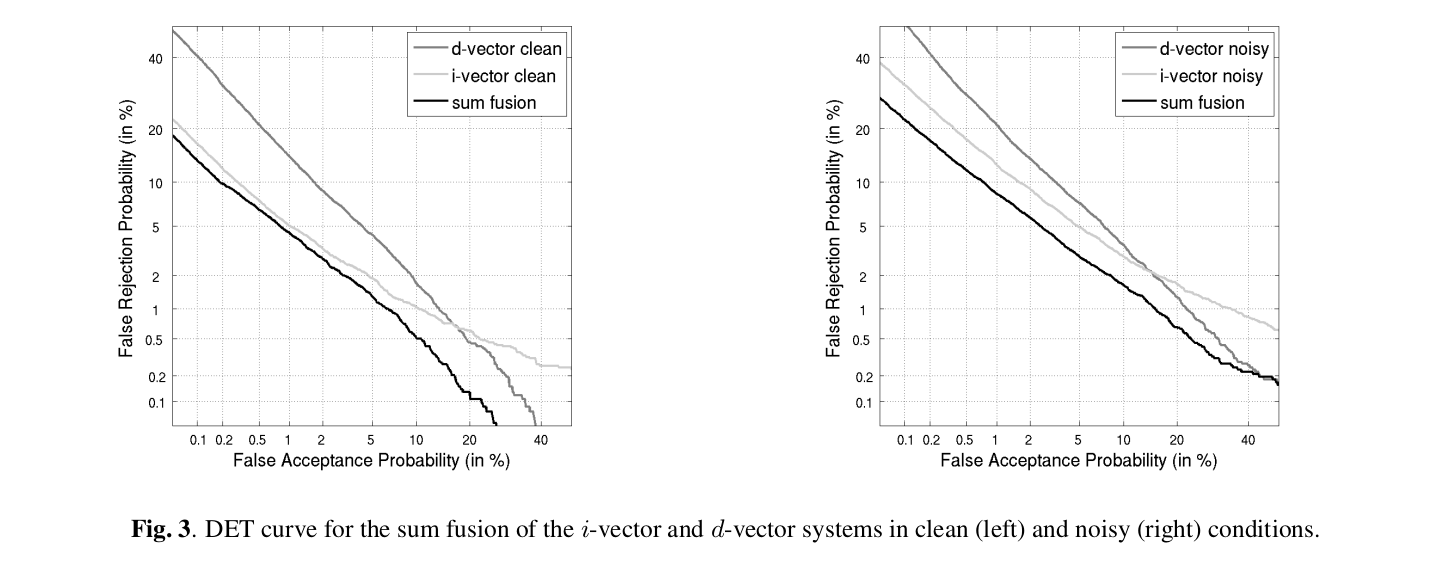
\includegraphics[width=0.85\linewidth]{images/i-vectors-d-vectors-det-sum-fusion.png}
		\caption{- Deep Neural Networks for small foot-print text-dependent speaker verification - 2014}
		\label{fig:writing-thesis}
	\end{figure}
	Tuy vậy, d-vectors vẫn cho ta nhiều hy vọng, kết quả khá khả quan về việc sử dụng DNN trong xác minh người nói
	
	\textbf{Nhận xét chung}
	\begin{itemize}
		\item Cơ sở của phương pháp có ý tưởng đơn giản là sử dụng Mạng Học Sâu trong việc rút trích đặc trưng và sử dụng lớp cuối cùng như một đặc trưng kích hoạt (deep vectors)
		\item Độ do dùng trong việc so sánh hai mô hình người nói đơn giản, so sánh cosine giữa hai vectors
		\item Kết quả có sự khả quan và nhiều hy vọng bằng chứng là xác suất đồng ý sai, từ chối sai thấp hơn hệ thống i-vectors trước đây
		\item EER vẫn chưa tốt so với hệ thống i-vectors
	\end{itemize}
	
	\subsubsection{D.2.5.2 Về j-vectors}
	\begin{figure}[H]
		\centering
		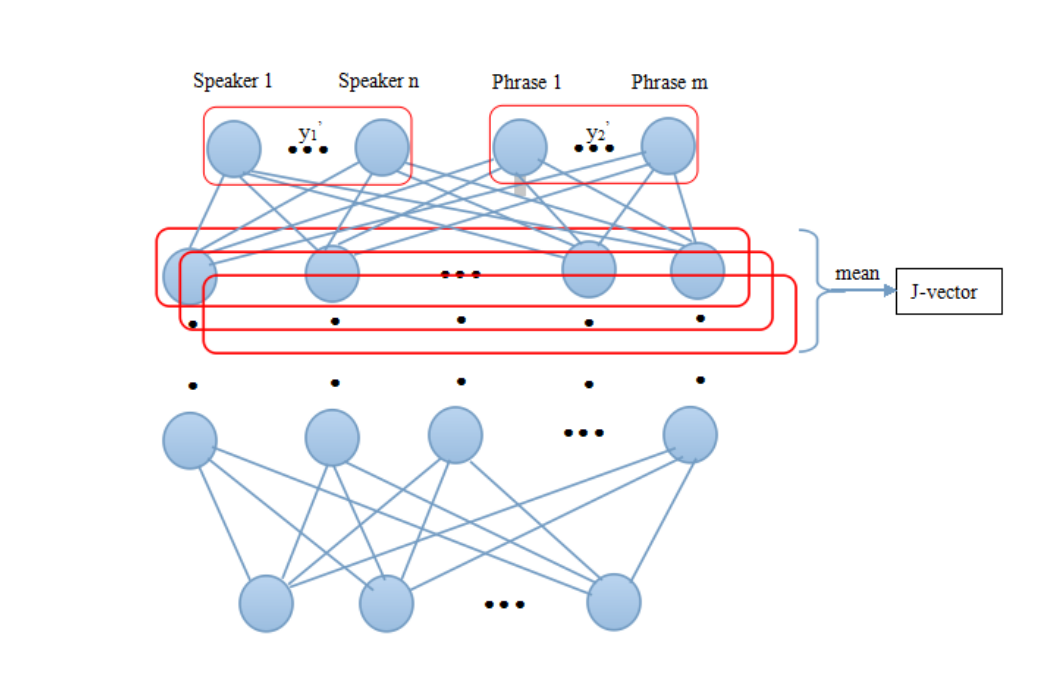
\includegraphics[width=0.75\linewidth]{images/j-vectors.png}
		\caption{Multi-task DNN in Multi-Task Learning for Text-Dependent Speaker Verification, 2014.}
		\label{fig:writing-thesis}
	\end{figure}
	\qquad Phương thức tiếp cận \textbf{d-vectors} được giới thiệu trong bài báo "Deep neural networks for small footprint text-dependent speaker verification" năm 2014 được mở rộng bằng phương thức tiếp cận học đa nhiệm (multi-task learning approach) và khái niệm về \textbf{j-vectors} được đưa ra, j-vectors có nghĩa là joint-vectors.
	
	\textbf{Giới thiệu chung về bài báo:}
	\begin{itemize}
		\item Bài báo: Multi-Task Learning for Text-Dependent Speaker Verification
		\item Nhóm tác giả: Nanxin Chen, Yanmin Qian, Kai Yu (Shanghai Jiao Tong University, China)
		\item Được publish tại hội nghị INTERSPEECH 2015 16th Annual Conference of the International Speech Communication Association, diễn ra tại Dresden, Germany, từ ngày 6-10 tháng 9 năm 2015
		\item Từ khóa: Deep neural network, Multi-task learning (Học đa nhiệm), Speaker verification (Xác minh người nói), Discriminant analysis (Phân tích phân tách), Probabilistic linear discriminant analysis (Phân tích xác suất phân tách tuyến tính), Deep learning (Học Sâu)
	\end{itemize}

	\textbf{Phương pháp}
	Mô hình Học đa nhiệm Deep Neural Network sử dụng cho Xác minh người nói phụ thuộc văn bản được lấy ý tưởng từ việc sử dụng DNN với số lượng tham số cực lớn, một mô hình DNN có thể học cùng lúc việc phân tách văn bản, lẫn giọng nói
	
	Hai hàm mất mát ban đầu là $C_1(y_1, y_1'), C_2(y_2, y_2')$ được dùng để tạo thành hàm tổng mất mát:
	$$C([y_1, y_2], [y_1', y_2']) = C_1(y_1, y_1') + C_2(y_2, y_2')$$
	Trong đó:
	\begin{itemize}
		\item $C_1, C_2$ lần lượt là hai cross-entropy criteria cho giọng nói và văn bản
		\item $y_1, y_2$ đại diện cho nhãn đúng của từng người nói và văn bản
		\item $y_1', y_2'$ đại diện cho nhãn đầu ra (nhãn dự đoán được) của $y_1, y_2$ tương ứng
	\end{itemize}
	
	Mỗi khi tiến trình của multi-task neural network huấn luyện xong, lớp output sẽ bị loại bỏ, phần còn lại của neural network sẽ được dùng để rút trích biểu diễn kết hợp giữa giọng nói và văn bản (sử dụng lớp ẩn cuối cùng) sau đó lấy trung bình, gọi là \textbf{j-vectors} (hay \textbf{joint-vector}) điểm này khá tương tự với d-vectors
	
	Có nhiều độ đo có thể sử dụng trong giai đoạn đăng ký, ở bài báo này, nhóm tác giả trình bày 2 cách thực hiện
	\begin{itemize}
		\item Joint Gaussian Discriminant Function
		$$\mathit{N}(x|\mu_k,\Sigma_k) = \frac{1}{(2\pi)^{\frac{p}{2}}|\Sigma_k|^{\frac{1}{2}}}e^{-\frac{1}{2}(x-\mu_k)^T\Sigma^{-1}(x-\mu_k)}$$
		Trong đó:
		\begin{itemize}
			\item $\Sigma_k$ là hiệp phương sai lớp k
			\item $\mu_k$ là trung bình lớp k
			\item $p$ là số chiều của vector
		\end{itemize}
		Mô hình LDA giả định rằng $\Sigma_k = \Sigma$, nhóm tác giả cho biết hàm discriminant function cho lớp thứ k như sau:
		$$df_k(x) = -\frac{1}{2} \times (x - \mu_k)^T\Sigma^{-1}(x-\mu_k)$$
		Và do trên trường hợp tập đóng, biểu thức có thể được rút gọn do giá trị $x^T\Sigma x$ có giá trị như nhau trên mọi lớp. Ta có một biểu thức tuyến tính (GDF)
		$$df_k' = (\Sigma^{-1}\mu_k)x + \left(-\frac{1}{2}\mu_k^T\Sigma^{-1}\mu_k\right)$$
		\item Probabilistic Linear Discriminant Analysis
		$$P(\mu_k) = N(\mu_k|m, \theta_b)$$
	\end{itemize}
	\textbf{Các kết quả}
	\begin{figure}[H]
		\centering
		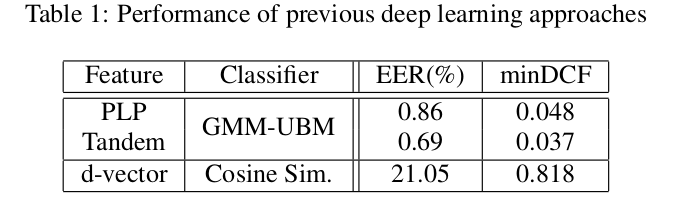
\includegraphics[width=0.75\linewidth]{images/j-vectors-table-01.png}
		\caption{Multi-task DNN in Multi-Task Learning for Text-Dependent Speaker Verification, 2014.}
		\label{fig:writing-thesis}
	\end{figure}
	\begin{figure}[H]
		\centering
		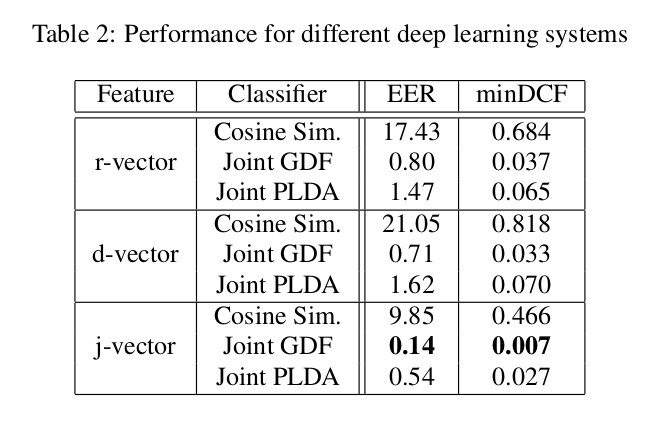
\includegraphics[width=0.75\linewidth]{images/j-vectors-result-table-02.png}
		\caption{Multi-task DNN in Multi-Task Learning for Text-Dependent Speaker Verification, 2014.}
		\label{fig:writing-thesis}
	\end{figure}
	\begin{figure}[H]
		\centering
		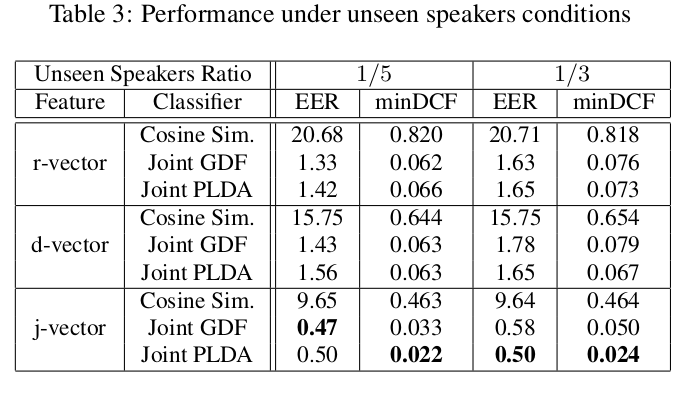
\includegraphics[width=0.75\linewidth]{images/j-vectors-result-table-03.png}
		\caption{Multi-task DNN in Multi-Task Learning for Text-Dependent Speaker Verification, 2014.}
		\label{fig:writing-thesis}
	\end{figure}
	\begin{figure}[H]
		\centering
		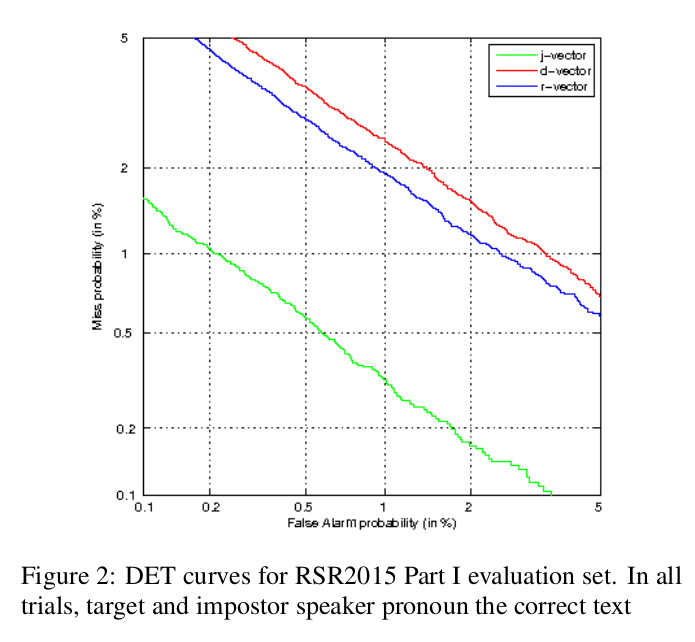
\includegraphics[width=0.75\linewidth]{images/j-vectors-fig-2.png}
		\caption{Multi-task DNN in Multi-Task Learning for Text-Dependent Speaker Verification, 2014.}
		\label{fig:writing-thesis}
	\end{figure}
	
	\textbf{Nhận xét}
	\begin{itemize}
		\item Bài báo đề xuất một framework sử dụng kỹ thuật Deep Learning cho tác vụ xác minh người nói phụ thuộc văn bản có kết quả hết sức có triển vọng
		\item Áp dụng học đa nhiệm (giọng nói và văn bản), rút trích ra j-vectors
		\item Sử dụng Gaussian Discriminant Function và Probability Linear Discriminant Analysis, hai kỹ thuật mạnh trong việc phân lớp giọng nói
		\item Kết quả tốt hơn, cho độ lỗi thấp hơn rất nhiều so với d-vector, r-vector trên tác vụ xác minh người nói phụ thuộc văn bản
	\end{itemize}
	
	\subsubsection{D.2.5.3 Về x-vectors}
	\begin{figure}[H]
		\centering
		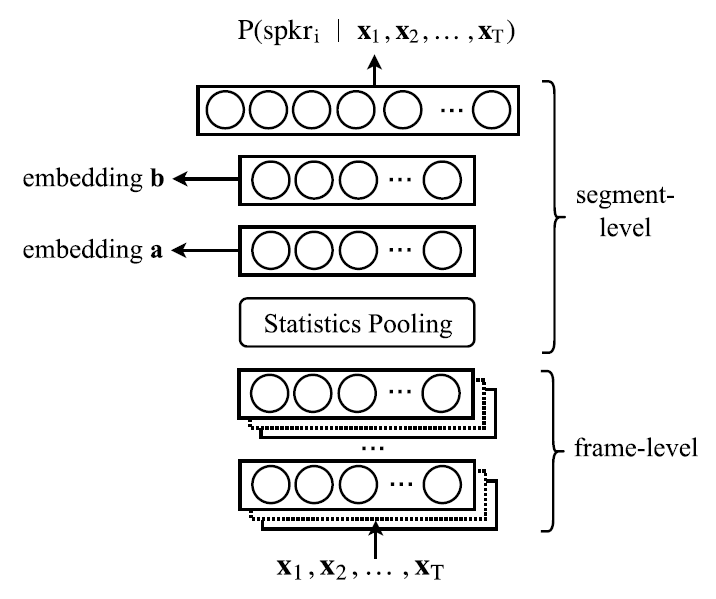
\includegraphics[width=0.75\linewidth]{images/x-vector.jpg}
		\caption{x-vector DNN embedding architecture in (Snyder et al., 2018)}
		\label{fig:writing-thesis}
	\end{figure}

	\textbf{Giới thiệu chung về bài báo:}
	\begin{itemize}
		\item Bài báo: X-Vectors: Robust DNN Embeddings for Speaker Recognition
		\item Nhóm tác giả: 
			\begin{itemize}
				\item \textbf{David Snyder} - Center for Language and Speech Processing \& Human Language Technology Center of Excellence, The Johns Hopkins University, Baltimore, MD, USA
				\item \textbf{Daniel Garcia-Romero} - Center for Language and Speech Processing \& Human Language Technology Center of Excellence, The Johns Hopkins University, Baltimore, MD, USA
				\item \textbf{Gregory Sell} - Center for Language and Speech Processing \& Human Language Technology Center of Excellence, The Johns Hopkins University, Baltimore, MD, USA
				\item \textbf{Daniel Povey} - Center for Language and Speech Processing \& Human Language Technology Center of Excellence, The Johns Hopkins University, Baltimore, MD, USA
				\item \textbf{Sanjeev Khudanpur} - Center for Language and Speech Processing \& Human Language Technology Center of Excellence, The Johns Hopkins University, Baltimore, MD, USA
			\end{itemize}
		\item Được xuất bản tại hội nghị 2018 IEEE International Conference on Acoustics, Speech and Signal Processing (ICASSP), diễn ra tại Calgary, AB, Canada, năm 2018
		\item Từ khóa: Speaker Recognition, Deep Neural Networks, Data Augmentation, x-vectors
	\end{itemize}
	
	\textbf{Phương pháp}
	\begin{figure}[H]
		\centering
		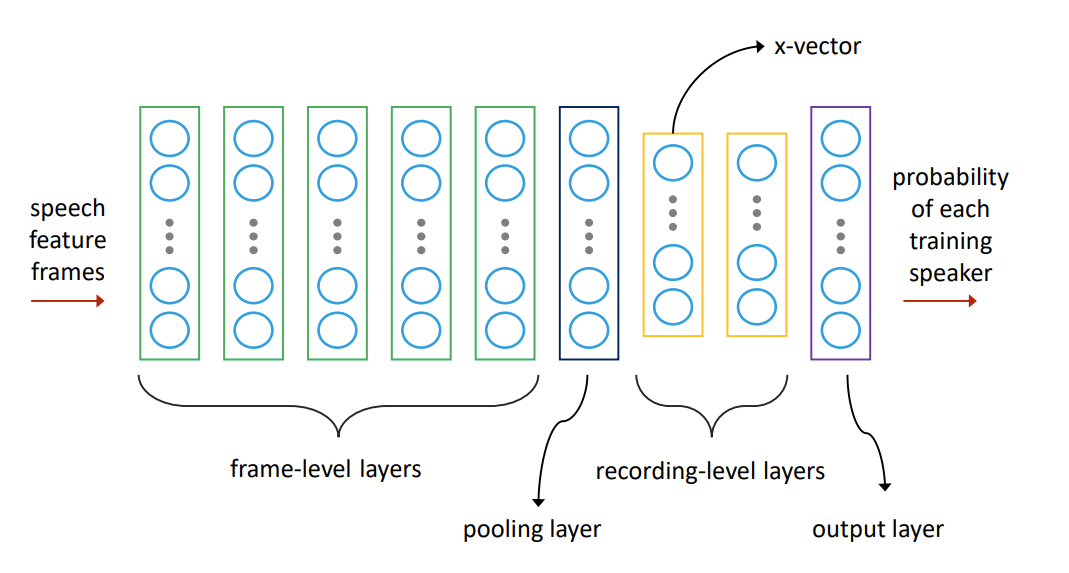
\includegraphics[width=0.75\linewidth]{images/x_vectors_dnn.png}
		\caption{x-vectors DNN - From i-vectors to x-vectors – a generational change in speaker recognition illustrated on the NFI-FRIDA database - OxfordWave Research}
		\label{fig:writing-thesis}
	\end{figure}
	Với 5 layers đầu tiên thực hiện tính toán trên các khung giọng nói với một ngữ cảnh thời gian nhỏ tập trung vào khung hiện tại, gọi là t. Ví dụ, đầu vào của frame2 là đầu ra của frame1, tại các frames t-2 và t + 2, thì tổng ngữ cảnh thời gian ở frame2 là 9
	
	Statistics pooling layer (lớp tổng hợp thống kê) tổng hợp tất cả các đầu ra ở mức khung T từ lớp frame5 và tính toán giá trị trung bình và độ lệch chuẩn của nó. Hai giá trị gồm giá trị trung bình và độ lệch chuẩn được kết lại, được đưa qua các lớp phân đoạn và cuối cùng qua lớp đầu ra softmax
	
	x-vectors sẽ được rút trích tại lớp phân đoạn 6 (segment6), ngay sau khi qua lớp tổng hợp thống kê
	
	\begin{figure}[H]
		\centering
		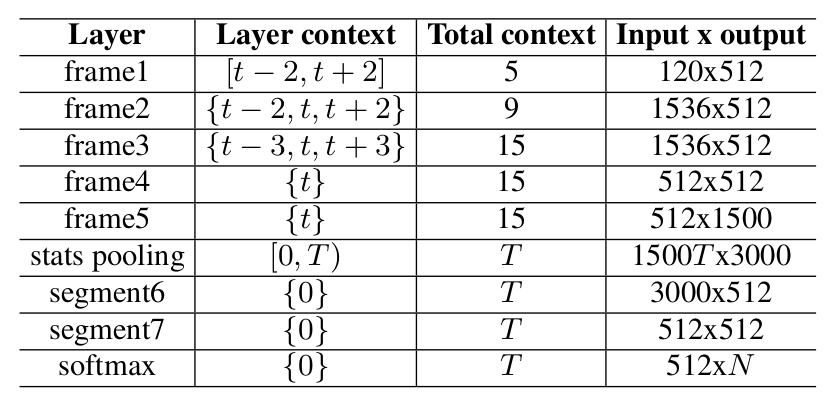
\includegraphics[width=0.75\linewidth]{images/x-vectors-setup.png}
		\caption{Configuration Table of x-vector DNN embedding architecture in (Snyder et al., 2018)}
		\label{fig:writing-thesis}
	\end{figure}

	Việc so sánh hai x-vector được mô hình như sau: Sử phân phối same-speaker và different speaker để ước lượng likelihood score để đưa ra so sánh hai vectors
	\begin{figure}[H]
		\centering
		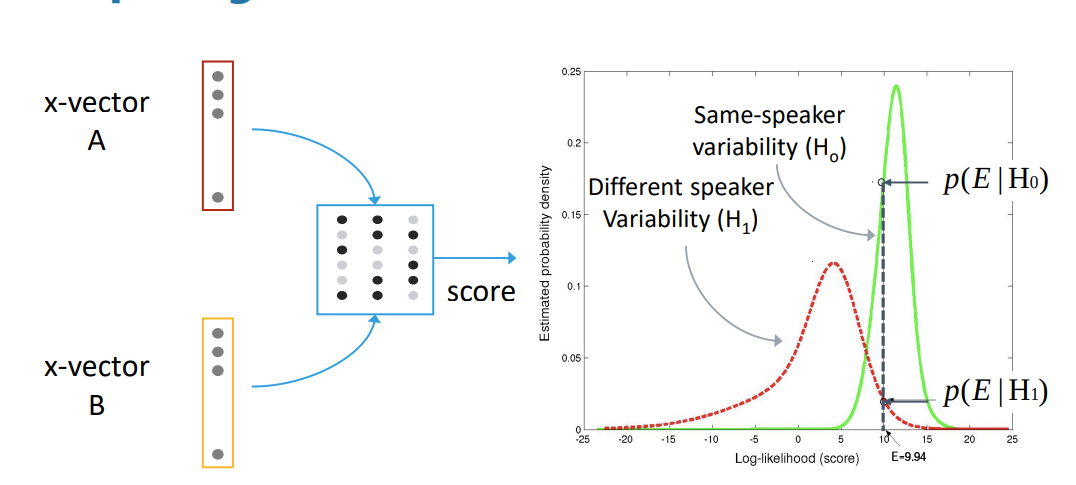
\includegraphics[width=0.75\linewidth]{images/comparing_x_vectors.png}
		\caption{x-vectors DNN - From i-vectors to x-vectors – a generational change in speaker recognition illustrated on the NFI-FRIDA database - OxfordWave Research}
		\label{fig:writing-thesis}
	\end{figure}

	\textbf{Các kết quả}
	\begin{figure}[H]
		\centering
		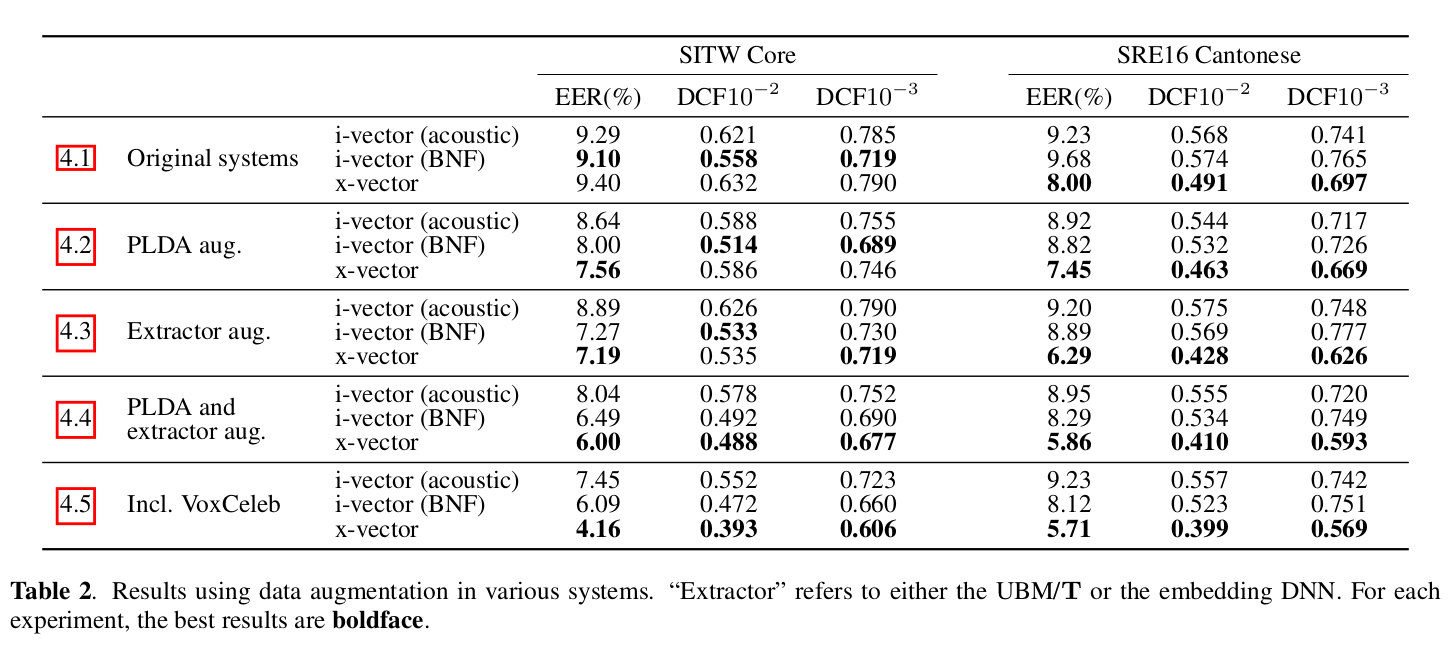
\includegraphics[width=1\linewidth]{images/x-vectors-result-table-02.png}
		\caption{x-vector DNN embedding architecture in (Snyder et al., 2018)}
		\label{fig:writing-thesis}
	\end{figure}
	\begin{figure}[H]
		\centering
		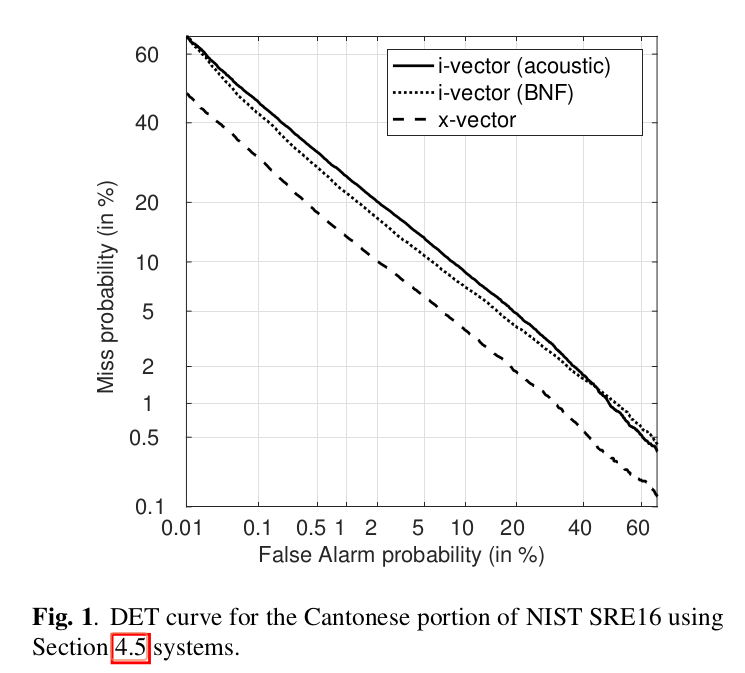
\includegraphics[width=0.75\linewidth]{images/x-vectors-fig-01.png}
		\caption{x-vector DNN embedding architecture in (Snyder et al., 2018)}
		\label{fig:writing-thesis}
	\end{figure}
	\begin{figure}[H]
		\centering
		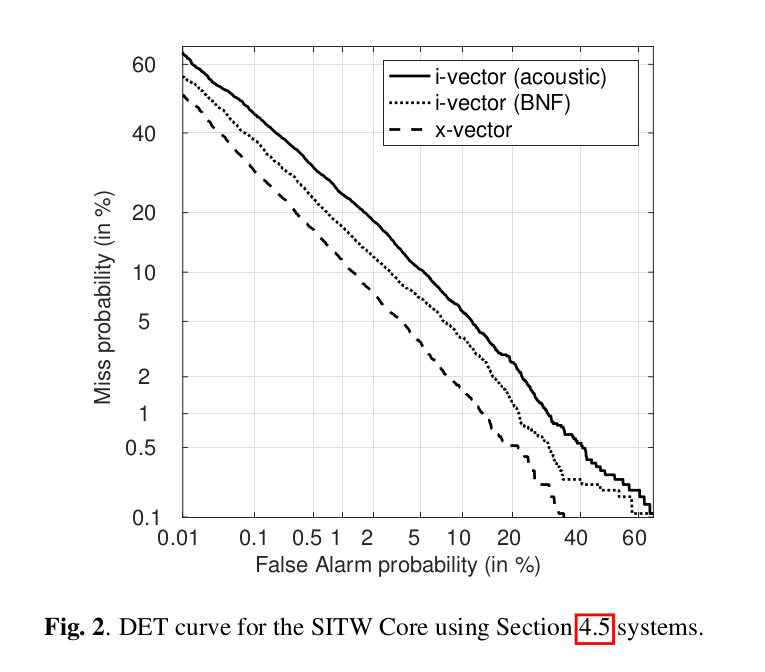
\includegraphics[width=0.75\linewidth]{images/x-vectors-fig-02.png}
		\caption{x-vector DNN embedding architecture in (Snyder et al., 2018)}
		\label{fig:writing-thesis}
	\end{figure}
	
	\textbf{Nhận xét}
	\begin{itemize}
		\item Hiệu suất của x-vectors đã được chứng minh là tốt hơn đáng kể so với i-vectors, đặc biệt là ở khoảng thời gian ngắn.
		\item Học có giám sát, x-vectors DNN được huấn luyện bằng cách dùng dữ liệu có nhãn người nói
		\item DNN x-vector có khả năng khai thác lượng dữ liệu huấn luyện lớn hơn so với khung i-vector, nó bão hòa sau một lượng dữ liệu huấn luyện nhất định.
		\item khả năng khai thác lượng dữ liệu huấn luyện lớn hơn cũng tạo điều kiện cho một phương pháp thúc đẩy số lượng và tính đa dạng của dữ liệu huấn luyện được gọi là tăng cường dữ liệu. Quá trình này thêm tiếng ồn và nhiễu vào các mẫu huấn luyện và đưa chúng vào huấn luyện cùng với các mẫu ban đầu.
		\item Khả năng sử dụng cùng front-end (trích xuất đặc trưng) và back-end (so sánh vector) cho cả hệ thống i-vectơ và x-vectơ tạo điều kiện tích hợp hệ thống và cho phép so sánh trực tiếp hơn giữa hai phương pháp mô hình hóa.
	\end{itemize}
	
	\subsubsection{D.2.5.4 So sánh d-vectors, j-vectors và x-vectors}
		\begin{table}[H]
		\centering
		\begin{tabular}{ |p{2cm} |p{4cm} | p{4cm} | p{4cm}  |}\hline
			& d-vectors & j-vectors & x-vector \\\hline
			Kỹ thuật rút trích & DNN & DNN & DNN\\ \hline
			Ví trí rút trích & Tại lớp ẩn cuối cùng DNN & Tại lớp ẩn cuối cùng DNN & Sau khi qua lớp statistics pooling\\\hline
			Cách rút trích & Là trung bình kích hoạt tại lớp ẩn cuối cùng & Là trung bình kích hoạt tại lớp ẩn cuối cùng, kết hợp tín hiệu giọng nói và dữ liệu văn bản & Là vector phân đoạn (segment6) sau khi tính toán thống kê\\\hline
		\end{tabular}
	\end{table}
	\subsection{D.2.5 Học Sâu trong tác vụ phân lớp giọng nói}
	\subsubsection{D.2.5.1 Multi-domain features}
	\textbf{Giới thiệu chung về bài báo:}
	\begin{itemize}
		\item Tên bài báo: Multi-task Recurrent Model for Speech and Speaker Recognition
		\item Nhóm tác giả: Zhiyuan Tang (1) (2) , Lantian Li (1) and Dong Wang (1)
		\begin{itemize}
			\item (1): Center for Speech and Language Technologies, Division of Technical Innovation and Development,
			Tsinghua National Laboratory for Information Science and Technology
			Center for Speech and Language Technologies, Research Institute of Information Technology, Tsinghua University
			\item (2): Chengdu Institute of Computer Applications, Chinese Academy of Sciences
		\end{itemize}
		\item Bài báo được đăng trên arXiv.org, vào ngày 31, tháng 3 năm 2016 (Phiên bản mới nhất được cập nhật vào ngày 27 tháng 9 năm 2016)
		\item Từ khóa: Multi-task, Recurrent Model, Speaker Recognition, 
	\end{itemize}
	\textbf{Phương pháp}
	\begin{figure}[H]
		\centering
		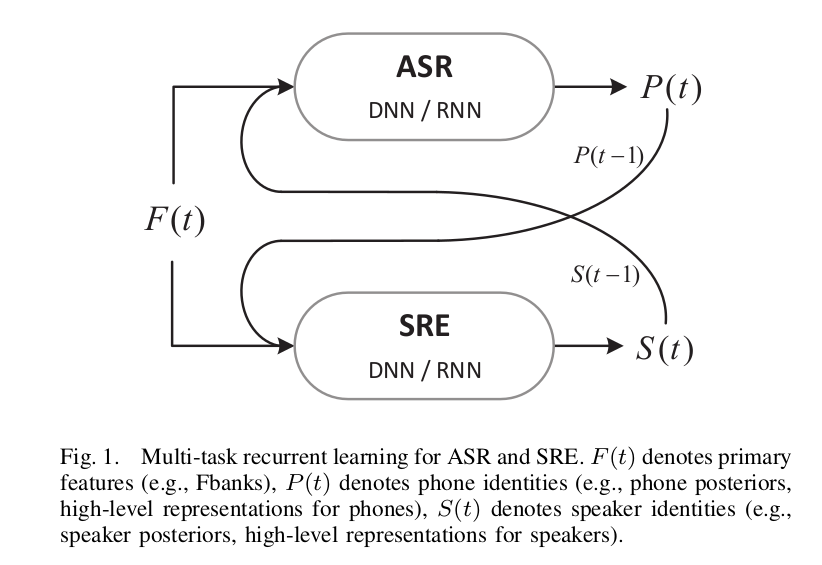
\includegraphics[width=0.75\linewidth]{images/multi-task-recurrent-learning.png}
		\label{fig:writing-thesis}
	\end{figure}
	\textbf{Single-task model}
	\begin{figure}[H]
		\centering
		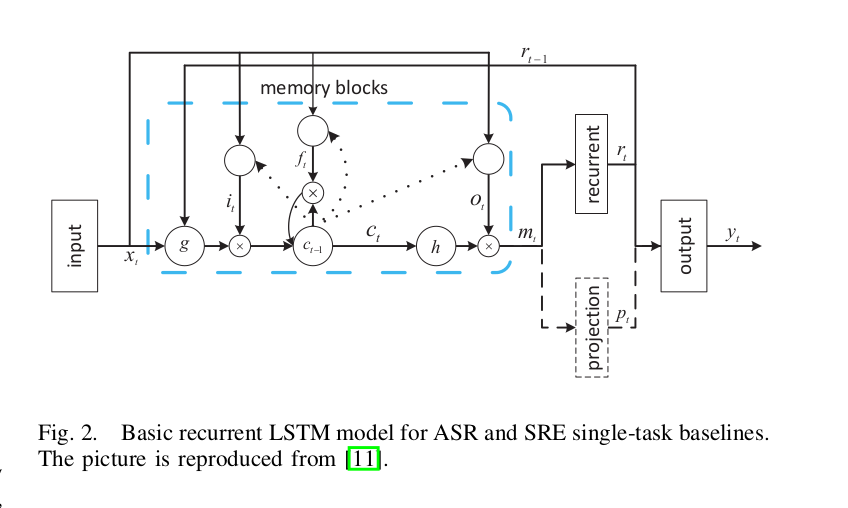
\includegraphics[width=0.75\linewidth]{images/basis-single-task-model.png}
		\label{fig:writing-thesis}
	\end{figure}
	\begin{gather*}
		i_t = \sigma(W_{ix}x_t + W_{ir}r_{t-1} + W_{ic}c_{t-1}=b_i)\\
		f_t = \sigma(W_{fx}x_t + W_{fr}r_{t-1} + W_{fc}c_{t-1}+b_f)\\
		c_t = f_t \odot c_{t-1} + i_t \odot g(W_{cx}x_t + W_{cr}r_{t-1} + b_c)\\
		o_t = \sigma(W_{ox}x_t + W_{or}r_{t-1} + W_{oc}c_t + b_o)\\
		m_t = o_t \odot h(c_t)\\
		r_t = W_{rm}m_t\\
		p_t = W_{pm}m_t\\
		y_t = W_{yr}r_t + W_{yp}p_t + b_y\\
	\end{gather*}
	\textbf{Multi-task model}
	\begin{figure}[H]
		\centering
		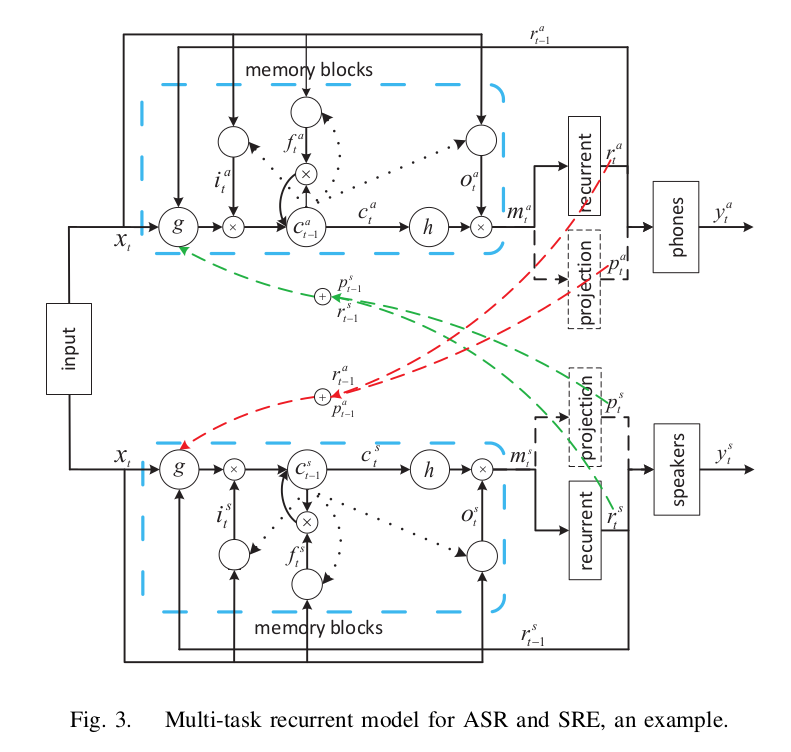
\includegraphics[width=0.75\linewidth]{images/multi-task-recurrent-model.png}
		\label{fig:writing-thesis}
	\end{figure}
	\textbf{Speech recognition (ASR)}
	\begin{gather*}
		i^{\alpha}_t = \sigma(W^{\alpha}_{ix}x_t + W^{\alpha}_{ir}r^{\alpha}_{t-1} + W^{\alpha}_{ic}c^{\alpha}_{t-1}+b^{\alpha}_i)\\
		f^{\alpha}_t = \sigma(W_{fx}x_t + W_{fr}r_{t-1} + W_{fc}c_{t-1}+b_f)\\
		g^{\alpha}_t = g(W^{\alpha}_{cx}x^{\alpha}_t + W^{\alpha}_{cr}r^{\alpha}_{t-1} + b^{\alpha}_{c} + \underline{W^{\alpha s}_{cr}r^{s}_{t-1} + W^{\alpha s}_{cp}p^{s}_{t-1}})\\
		c^{\alpha}_t = f_t \odot c_{t-1} + i_t \odot g(W_{cx}x_t + W_{cr}r_{t-1} + b_c)\\
		o^{\alpha}_t = \sigma(W^{\alpha}_{ox}x^{\alpha}_t + W^{\alpha}_{or}r^{\alpha}_{t-1} + W^{\alpha}_{oc}c^{\alpha}_t + b^{\alpha}_o)\\
		m^{\alpha}_t = o^{\alpha}_t \odot h(c^{\alpha}_t)\\
		r^{\alpha}_t = W^{\alpha}_{rm}m^{\alpha}_t\\
		p^{\alpha}_t = W^{\alpha}_{pm}m^{\alpha}_t\\
		y^{\alpha}_t = W^{\alpha}_{yr}r^{\alpha}_t + W^{\alpha}_{yp}p^{\alpha}_t + b^{\alpha}_y\\
	\end{gather*}
	\textbf{Speaker recognition (SRE)}
	\begin{gather*}
		i^{s}_t = \sigma(W^{s}_{ix}x_t + W^{s}_{ir}r^{s}_{t-1} + W^{s}_{ic}c^{s}_{t-1}+b^{s}_i)\\
		f^{s}_t = \sigma(W_{fx}x_t + W_{fr}r_{t-1} + W_{fc}c_{t-1}+b_f)\\
		g^{s}_t = g(W^{s}_{cx}x^{s}_t + W^{s}_{cr}r^{s}_{t-1} + b^{s}_{c} + \underline{W^{s\alpha}_{cr}r^{s}_{t-1} + W^{s\alpha}_{cp}p^{s}_{t-1}})\\
		c^{s}_t = f_t \odot c_{t-1} + i_t \odot g(W_{cx}x_t + W_{cr}r_{t-1} + b_c)\\
		o^{s}_t = \sigma(W^{s}_{ox}x^{s}_t + W^{s}_{or}r^{s}_{t-1} + W^{s}_{oc}c^{s}_t + b^{s}_o)\\
		m^{s}_t = o^{s}_t \odot h(c^{s}_t)\\
		r^{s}_t = W^{s}_{rm}m^{s}_t\\
		p^{s}_t = W^{s}_{pm}m^{s}_t\\
		y^{s}_t = W^{s}_{yr}r^{s}_t + W^{s}_{yp}p^{s}_t + b^{s}_y\\
	\end{gather*}
	\textbf{Các kết quả}
	\begin{itemize}
		\item Dữ liệu
		\item ASR baseline
		\begin{figure}[H]
			\centering
			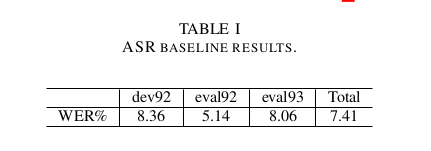
\includegraphics[width=0.5\linewidth]{images/multi-task-recurrent-model-asr-baseline-res.png}
			\label{fig:writing-thesis}
		\end{figure}
		\item SRE baseline
		\begin{figure}[H]
			\centering
			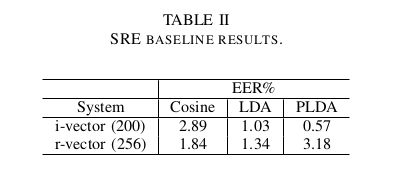
\includegraphics[width=0.5\linewidth]{images/multi-task-recurrent-model-sre-baseline-res.png}
			\label{fig:writing-thesis}
		\end{figure}
		\item Multi-task joint training
		\begin{figure}[H]
			\centering
			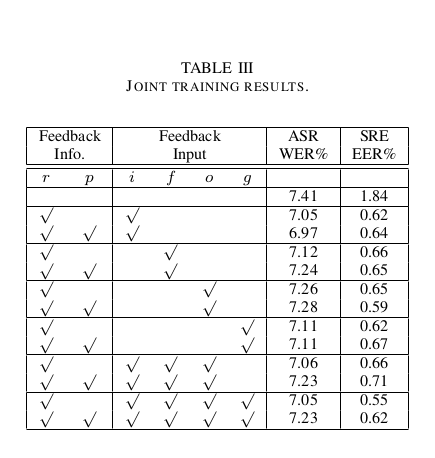
\includegraphics[width=0.5\linewidth]{images/multi-task-recurrent-model-joint-training-res.png}
			\label{fig:writing-thesis}
		\end{figure}
	\end{itemize}
	\textbf{Nhận xét}
	\begin{itemize}
		\item 
	\end{itemize}
	\subsubsection{D.2.5.1 SincNet}
	\qquad \textbf{Giới thiệu chung về bài báo}
	\begin{itemize}
		\item Nhóm tác giả trong bài báo này đề xuất một kiến trúc mạng CNN (Convolutional Neural Networks) mới, được gọi là SincNet, khai phá lớp tích chập đầu tiên để khám phá nhiều thông tin hơn. SincNet dựa trên các hàm $sinc$ được tham số hóa, để cài đặt các bộ lọc băng thông.
		\item Ngược lại với CNNs chuẩn, học tất cả các phần tử của mỗi bộ lọc filter, ở đây, chúng ta chỉ có các tần số cắt thấp và cao học trực tiếp dữ liệu với phương pháp đề xuất
		\item Cung cấp một tập các bộ lọc mà chúng nhỏ gọn và hiệu quả trong việc tùy chỉnh với ứng dụng mà chúng ta muốn.
		\item Một sự kết hợp tuyệt vời giữa hai lĩnh vực khoa học lớn: Học máy (Machine Learning) và Xử lý Tín hiệu số (Digital Signal Processing).
		\item Bài báo được đăng công khai trên \href{arxiv.org}{arXiv dot org} lần đầu tiên vào năm 2018 bởi hai người Mirco Ravanelli, Yoshua Bengio (ông được xem là một trong 3 vị cha đẻ của phương pháp Deep Learning hiện đại), phiên bản cập nhật gần đây nhất là vào năm 2019 bằng việc thay thế hàm "sinc\_conv" bằng "SincConv\_fast" giúp tăng tốc độ lên 50\% so với phiên bản cũ.
		\item Từ khóa: Speaker recognition, Convolutional Neural Networks, Raw samples
	\end{itemize}
	 
	\textbf{Vấn đề khi xử lý tín hiệu giọng nói: Dữ liệu đầu vào có số chiều cao}
	
	Convolutional Neural Networks - CNNs là một lựa chọn thích hợp với đầu vào là những sóng thô, nó kiến trúc phổ biến nhất để xử lý các mẫu giọng nói thô nhờ vào chia sẻ trọng số, bộ lọc cục bộ và tổng hợp giúp khám phá các biểu diễn dữ liệu và bất biến. Vấn đề lớn nhất đối với sóng thô dựa trên mạng CNNs chính là \textbf{lớp tích chập đầu tiên}.
	\begin{figure}[H]
		\centering
		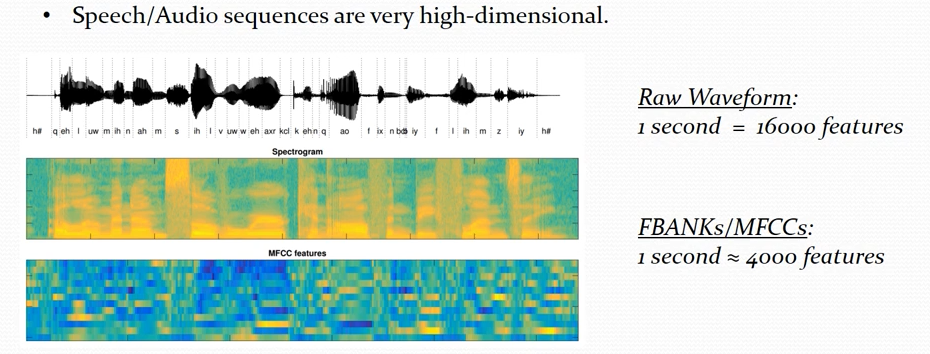
\includegraphics[width=1\textwidth]{images/capture_01.png}
		\caption{Minh họa chuỗi giọng nói có số chiều rất lớn. Ảnh được lấy từ video A bref introduction to SincNet thực hiện bởi Giáo sư Mirco Ravanelli}
		\label{fig:writing-thesis}
	\end{figure}
	Ở lớp này, dữ liệu đầu vào là những chuỗi Speech/Audio có số chiều rất cao, ví dụ như: cứ mỗi giây thì ta lại có đến 16000 đặc trưng. Bằng những kỹ thuật thủ công ngày xưa như FBANKs hay MFCCs thì ta có thể giúp nó giảm xuống còn 4000 đặc trưng mỗi giây, nhưng như thế vẫn còn rất nhiều!
	
	\textbf{Vấn đề khi xử lý tín hiệu giọng nói: Những thông tin nhận dạng (đặc trưng giọng nói) dễ bị mất đi}. Những đặc trưng trong phổ tần số có thể nhận ra bằng mắt thường nhưng lại bị mất đi nếu chúng ta làm mịn chúng bằng những kỹ thuật thủ công như FBANKs hay MFCCs.
	\begin{figure}[H]
		\centering
		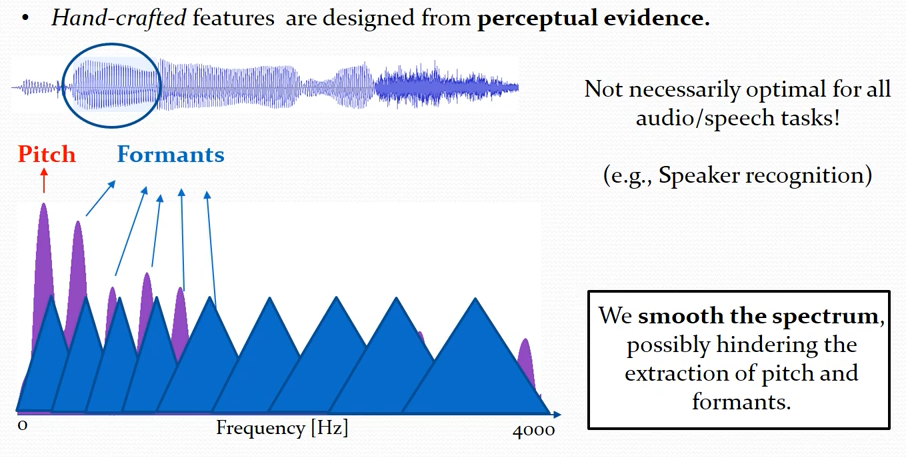
\includegraphics[width=1\textwidth]{images/perceptual_evidence.png}
		\caption{Ảnh được lấy từ video A bref introduction to SincNet thực hiện bởi Giáo sư Mirco Ravanelli}
		\label{fig:writing-thesis}
	\end{figure}
	
	\textbf{Vấn đề khi xử lý tín hiệu giọng nói: Vấn đề mất dốc đạo hàm - Một vấn đề thường gặp khi làm việc với Mạng học Sâu}. Không những gặp vấn đề về số chiều dữ liệu mà còn bị ảnh hưởng nhiều hơn bởi các vấn đề về sự biến mất độ dốc đạo hàm, đặc biệt là khi sử dụng các kiến trúc rất sâu.
	\begin{figure}[H]
		\centering
		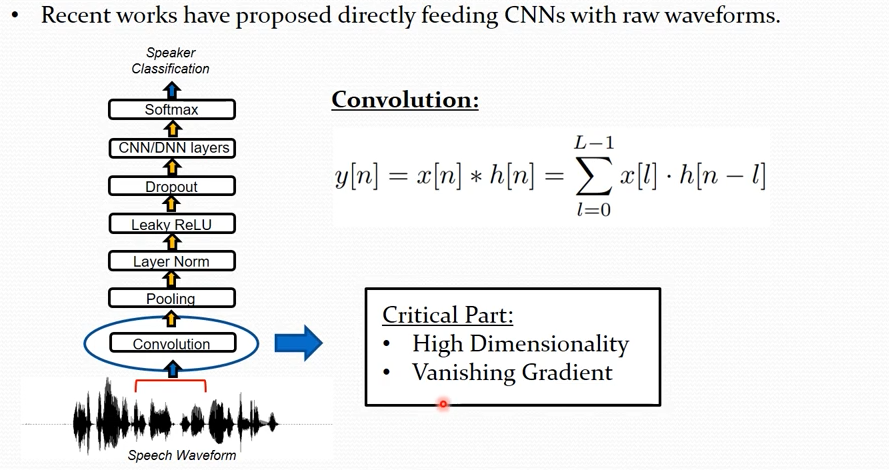
\includegraphics[width=1\textwidth]{images/cnns_problems.png}
		\caption{Ảnh được lấy từ video A bref introduction to SincNet thực hiện bởi Giáo sư Mirco Ravanelli}
		\label{fig:writing-thesis}
	\end{figure}
	
	\begin{figure}[H]
		\centering
		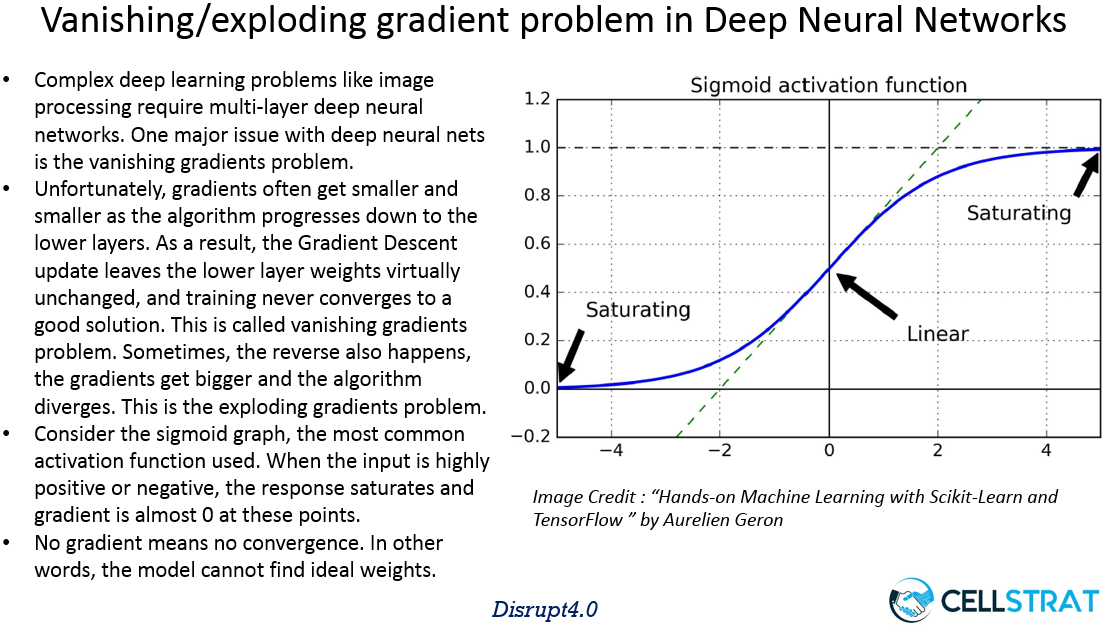
\includegraphics[width=1\textwidth]{images/Vanishing-Gradients-in-DNN.png}
		\caption{Vấn đề Vanishing Gradient trong Deep Neural Networks}
		\label{fig:writing-thesis}
	\end{figure}
	\textbf{Vấn đề khi xử lý tín hiệu giọng nói: Hình dạng của các bộ lọc CNN}. Ngoài ra, các bộ lọc CNNs thường có những hình dạng đa băng tần không hợp lý, để hiểu nó thì với mạng Neural là điều dễ dàng, nhưng với con người thì nó không có nhiều ý nghĩa trong việc thể hiện giọng nói.
	\begin{figure}[H]
		\centering
		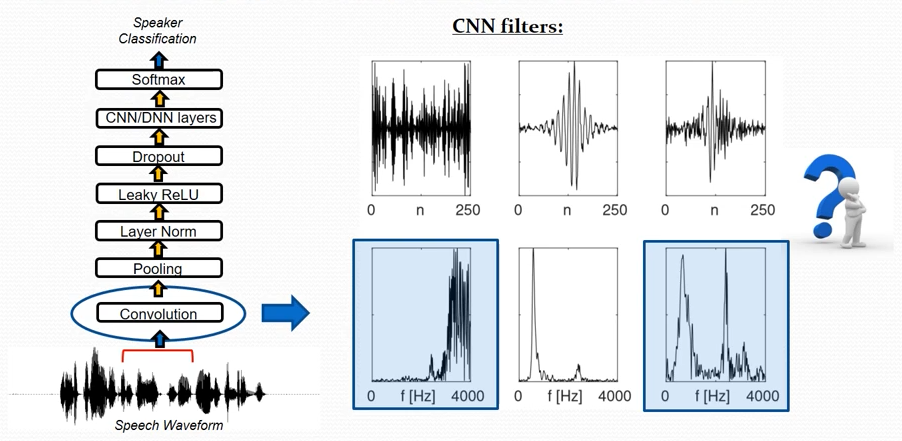
\includegraphics[width=1\textwidth]{images/interpretability_problems.png}
		\caption{Ảnh được lấy từ video A bref introduction to SincNet thực hiện bởi Giáo sư Mirco Ravanelli}
		\label{fig:writing-thesis}
	\end{figure}

	\textbf{Những ý tưởng bắt nguồn từ Xử lý tín hiệu số và điều chỉnh lại CNN chuẩn}
	
	Với một CNN chuẩn, việc tích chập trong miền thời gian giữa input waveform và một số đáp ứng xung hữu hạn (Finite Impulse Response - FIR) được cho bởi công thức:
	
	$$y[n] = x[n] * h[n] = \sum_{l=0}^{L-1}x[l].h[n-l]$$ 
	
	Trong đó:
	\begin{itemize}
		\item $x[n]$: đoạn tín hiệu giọng nói
		\item $h[n]$: một mặt nạ ứng với chiều dài $L$
		\item $y[n]$: giá trị đầu ra
	\end{itemize}
	
	Trong khi đó, Sincnet thực hiện các phép tích chập của nó với hàm $g$, hàm này phụ thuộc vào một tham số $\theta$. Công thức như sau:
	
	$$y[n] = x[n] * g[n, \theta]$$
	
	Trong xử lý tín hiệu số, $g$ được định nghĩa như một filter-bank gồm các bộ lọc (filter) băng thông hình chữ nhật. Trong miền tần số, độ lớn của một bộ lọc băng thông tổng quát có thể được tính như hiệu số giữa 2 bộ lọc thông tần số thấp
	
	Với $f_1$ $f_2$ lần lượt là tần số cắt thấp (low) và cao (high) đã được học, $rect(.)$ là hàm rectangular trong miền tần số.
	
	$$G[f, f_1, f_2] = rect\left(\frac{f}{2f_2}\right) -  rect\left(\frac{f}{2f_1}\right)$$
	
	Công thức trên đang ở trong miền tần số, để có thể trở lại miền thời gian được, ta sử dụng phép biến đổi Fourier Ngược
	
	Note: Biến đổi Fourier cho hàm Rectangular
	
	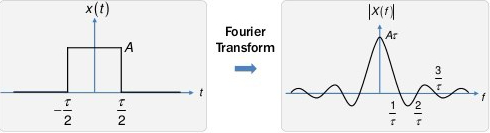
\includegraphics[width=1\textwidth]{images/rect_fourier.jpg}\\
	
	$$x(t) = Arect(\frac{t}{\tau})$$
	
	Biến đổi:
	
	$$X(\omega) = \int_{-\infty}^{\infty} x(t)e^{-j \omega t}\;\mathrm{d}t 
	$$
	
	$$X(\omega) = \int_{-\frac{\tau}{2}}^{\frac{\tau}{2}} Ae^{-j \omega t}\;\mathrm{d}t 
	= -\frac{2A}{\omega}\left[\frac{e^{-\frac{j \omega \tau}{2}} - e^{\frac{j \omega \tau}{2}}}{2j}\right]
	= \frac{2A}{\omega} \left[sin\left(\frac{\omega \tau}{2}\right)\right]
	= A\tau \left[\frac{sin(\frac{\omega \tau}{2})}{\frac{\omega \tau}{2}}\right]
	$$
	
	Hàm $sinc$ được định nghĩa
	
	$$sinc(x) = \frac{sin(x)}{x}$$
	
	Theo đó:
	
	$$X(\omega) = A\tau sinc\left(\frac{\omega \tau}{2}\right)$$
	
	Áp dụng công thức:
	
	Biến đổi ngược:
	
	$$G[f, f_1, f_2] = rect\left(\frac{f}{2f_2}\right) -  rect\left(\frac{f}{2f_1}\right)$$
	
	Ta được hàm tham chiếu $g$
	
	$$g[n, f_1, f_2] = 2f_2sinc(2\pi f_2 n) - 2f_1sinc(2\pi f_1 n)$$ 
	
	Các tần số cắt (cut-off frequencies) có thể được khởi tạo một cách ngẫu nhiên trong khoảng $\left[0, \frac{f_2}{2}\right]$, trong đó $f_s$ là tần số mẫu của tín hiệu đầu vào.
	
	Tần suất lấy mẫu có thể thay đổi theo loại dữ liệu chúng ta đang thử nghiệm. Hệ thống IVR có tần số lấy mẫu là 8Khz, trong khi hệ thống âm thanh nổi có tần số lấy mẫu là 44khz.
	
	Chúng ta có thể khởi tạo các bộ lọc dựa trên các tần số cắt của bộ lọc mel-scale filter-bank. Ưu điểm chính của việc chỉ định bộ lọc theo cách này là nó có lợi thế là phân bổ trực tiếp nhiều bộ lọc hơn ở phần dưới của phổ có thông tin duy nhất về giọng nói của người nói.
	
	Để đảm bảo $f1 \geq 0$ và $f_2 \geq f_1$, phương trình phía trên được cung cấp bởi các tham số sau:
	
	$$f_{1}^{abs} = |f_1|$$
	
	$$f_{2}^{abs} = f_1 + |f_2 - f_1| $$
	
	Ở đây, không có giới hạn nào đối với $f_2$, tức là không có tác nhân nào tác động lên $f_2$ để nó có thể nhỏ hơn tần số Nyquist (tốc độ tối thiểu mà tín hiệu có thể được lấy mẫu mà không có lỗi, gấp đôi tần số cao nhất hiện có trong tín hiệu) như mô hình học điều này trong khi huấn luyện. Các lớp tiếp theo khác nhau quyết định mức độ quan trọng nhiều hơn hoặc ít hơn cho mỗi đầu ra bộ lọc.
	
	Bộ lọc băng thông lý tưởng cần có vô số phần tử $L$. Một bộ lọc băng thông lý tưởng là nơi băng thông hoàn toàn phẳng và độ suy giảm trong băng thông dừng là vô hạn. Bất kỳ sự cắt ngắn nào của $g$ chắc chắn dẫn sẽ đến sự xấp xỉ của bộ lọc lý tưởng, được đặc trưng bởi các gợn sóng trong băng thông và suy giảm giới hạn dừng băng thông.
	
	Vì vậy, giải pháp cửa sổ (windowing) được thực hiện để giải quyết vấn đề này. Nó được thực hiện chỉ bằng cách nhân hàm bị cắt ngắn $g$ với cửa sổ $w$, nhằm mục đích làm phẳng các điểm gián đoạn đột ngột ở cuối $g$
	
	$$g_{w}\left[n, f_1, f_2\right] = g[n, f_1, f_2 . w[n]$$
	
	Trong bài báo, tác giả sử dụng Hamming Window, được định nghĩa bởi công thức:
	
	$$w[n] = 0.54 - 0.46.cos(\frac{2\pi n}{L})$$
	
	
	Chúng ta có thể có được tính chọn lọc tần số cao với việc sử dụng cửa sổ Hamming. Chúng ta cũng có thể sử dụng các cửa sổ khác như Hann, Blackman, Kaiser window. Một lưu ý quan trọng ở đây là do tính đối xứng, các bộ lọc có thể được tính toán hiệu quả bằng cách xem xét một nửa bộ lọc và kế thừa kết quả cho nửa còn lại.
	
	Tần số cắt của các bộ lọc có thể được tối ưu với các thông số CNN sử dụng Stochastic Gradient Descent (SGD) hoặc các phương pháp tối ưu Gradient khác. Như mô hình bên dưới, CNN pipeline (Pooling, Normalization, Activations, Dropout) có thể được sử dụng sau tích chập dựa trên Sinc Convolution đầu tiên. Multiple standard convolutional, fully-connehoặccted hoặc recurrent layers có thể đặt chồng lên ở giai đoạn sau đó để cuối cùng qua Softmax Classifier (Bộ phân lớp Softmax) để phân lớp giọng nói.
	
	\begin{figure}[H]
		\centering
		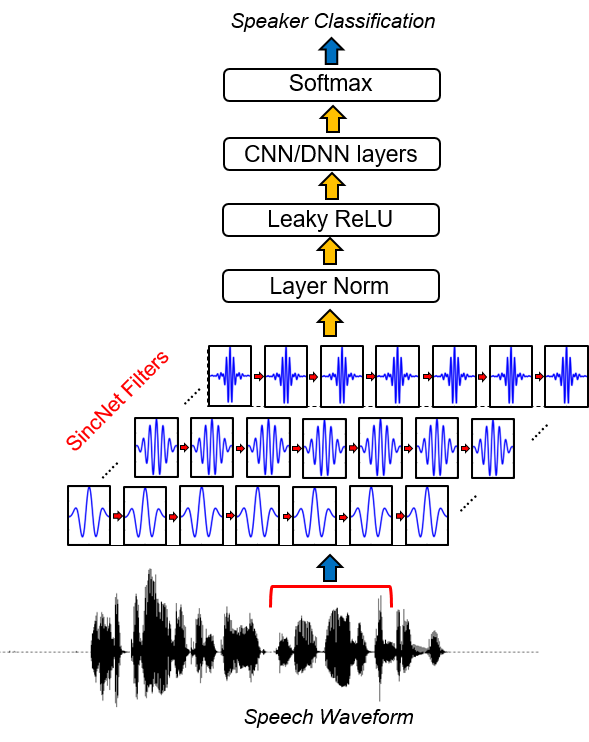
\includegraphics[width=0.75\textwidth]{images/SincNet.png}
		\caption{Kiến trúc mạng Sicnet}
		\label{fig:writing-thesis}
	\end{figure}
	
	
	\textbf{Đặc điểm của mô hình mạng SincNet}
	\begin{itemize}
		\item \textbf{Tính hội tụ nhanh}
		\begin{itemize}
			\item Sincnet được thiết kế theo cách mà nó buộc mạng phải tập trung vào các thông số lọc ảnh hưởng đến tốc độ của nó. Phong cách kỹ thuật lọc này giúp thích ứng với dữ liệu trong khi nắm bắt được tri thức giống như kỹ thuật trích xuất đặc trưng trên dữ liệu âm thanh. Tiền tri thức này làm cho việc học các đặc tính của bộ lọc dễ dàng hơn nhiều, giúp SincNet hội tụ nhanh hơn đáng kể đến một giải pháp tốt hơn. Chúng ta có được sự hội tụ nhanh chóng trong vòng 10–15 epochs đầu tiên.
			\begin{figure}[H]
				\centering
				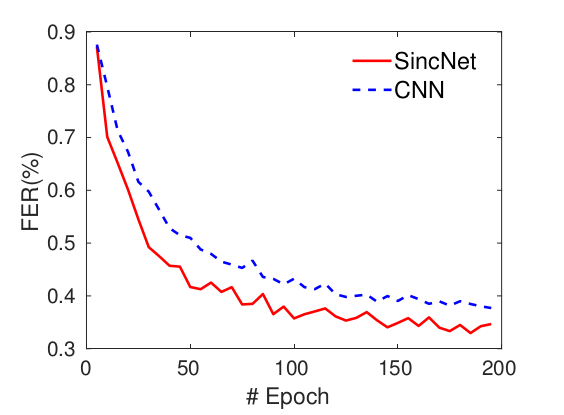
\includegraphics[width=0.4\textwidth]{images/fast_convergence.png}
				\caption{Độ hội tụ của SincNet so với CNN}
				\label{fig:writing-thesis}
			\end{figure}
		\end{itemize}
		\item \textbf{Tính hiệu quả}
		\begin{itemize}
			\item Do các hàm kernel $g(.)$ là đối xứng nên ta có thể thực hiện phép tích chập trên một phần filter và kế thừa kết quả này trên phần còn lại. Điều này sẽ tiết kiệm 50\% việc tính toán.
			\begin{figure}[H]
				\centering
				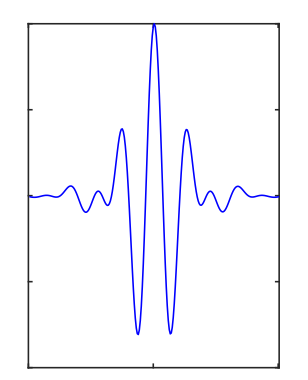
\includegraphics[width=0.3\textwidth]{images/g_symmetric.png}
				\caption{Hàm kernel}
				\label{fig:writing-thesis}
			\end{figure}
		\end{itemize}
		\item \textbf{Cần ít tham số cho việc huấn luyện mô hình}
		\begin{itemize}
			\item SincNet giảm đáng kể số lượng tham số trong lớp chập đầu tiên. Ví dụ: nếu chúng ta xem xét một lớp bao gồm các bộ lọc $F$ có độ dài $L$, một CNN tiêu chuẩn sử dụng các tham số $F * L$, so với $2F$ được SincNet xem xét. Nếu $F = 90$ và $L = 100$, chúng ta sử dụng $9000$ tham số cho CNN và chỉ $180$ cho SincNet. Hơn nữa, nếu chúng ta tăng gấp đôi độ dài bộ lọc $L$, một CNN chuẩn sẽ tăng gấp đôi số lượng tham số của nó (ví dụ: chúng ta đi từ $9000$ lên $18000$), trong khi SincNet có số lượng tham số không thay đổi (chỉ có hai tham số được sử dụng cho mỗi bộ lọc, bất kể độ dài $L$ của nó). Điều này cung cấp khả năng tạo ra các bộ lọc rất chọn lọc với nhiều lần nhấn, mà không thực sự thêm các tham số vào vấn đề tối ưu hóa. Hơn nữa, sự nhỏ gọn của kiến trúc SincNet làm cho nó phù hợp trong trường hợp ít mẫu.
		\end{itemize}
		\item \textbf{Tính giải nghĩa/ diễn giải}
		\begin{itemize}
			\item Các feature maps của SincNet sau khi thực hiện lớp tích chập đầu tiên rất dễ hiểu và con người có thể hiểu được so với những cách tiếp cận khác. Trên thực tế, các filter-bank chỉ phụ thuộc vào các tham số có ý nghĩa vật lý rõ ràng.
		\end{itemize}
		\begin{figure}[H]
			\centering
			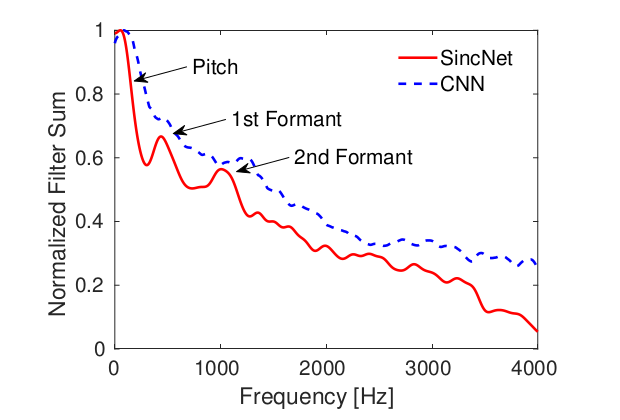
\includegraphics[width=0.5\textwidth]{images/interpretability.png}
			\caption{Khả năng diễn giải của SincNet so với CNN}
			\label{fig:writing-thesis}
		\end{figure}
		
		\begin{figure}[H]
			\centering
			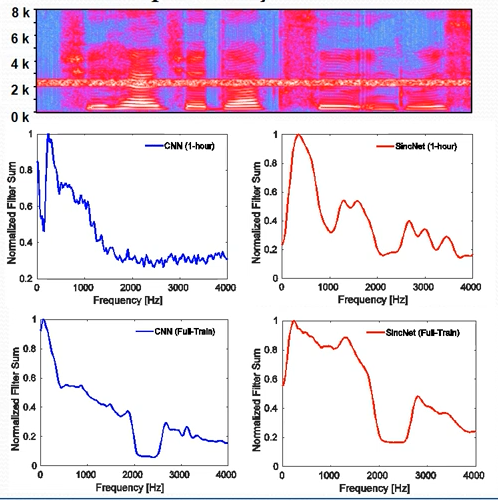
\includegraphics[width=.75\textwidth]{images/interpretability_2.png}
			\caption{Khả năng diễn giải của SincNet so với CNN}
			\label{fig:writing-thesis}
		\end{figure}
	\end{itemize}
	
	\textbf{Đối chiếu Convolution Neural Networks với SincNet}
	\begin{figure}[H]
		\centering
		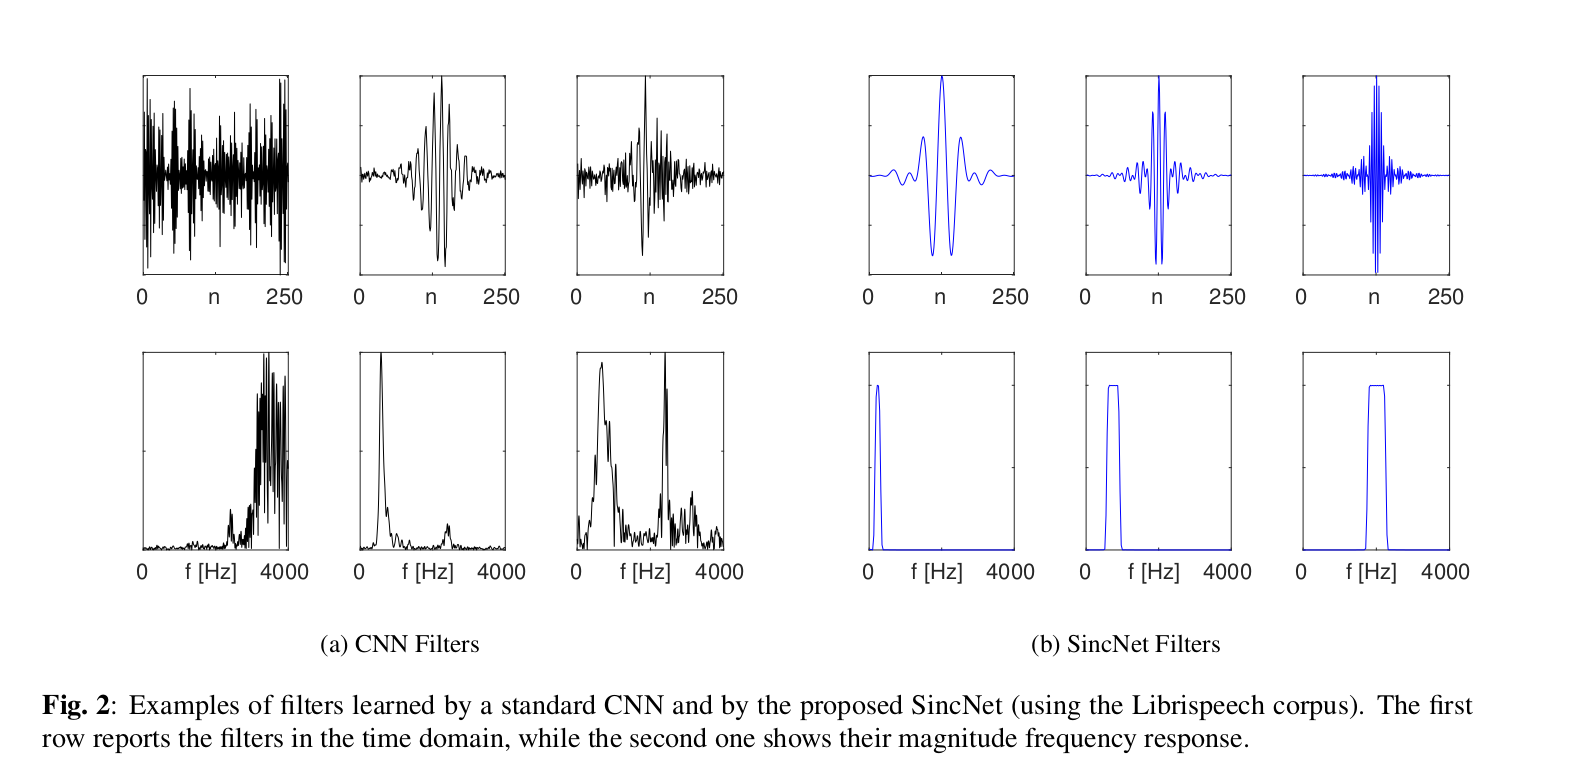
\includegraphics[width=1\textwidth]{images/cnn_filters_sincnet_filters.png}
		\caption{Ví dụ về các bộ lọc được học bởi CNN tiêu chuẩn và bởi SincNet (sử dụng kho ngữ liệu Librispeech). Hàng đầu tiên thể hiện các bộ lọc trong miền thời gian, trong khi hàng thứ hai hiển thị phản hồi tần số cường độ của chúng.}
		\label{fig:writing-thesis}
	\end{figure}

	\textbf{Các kết quả đối với tác vụ định danh người nói: }Như đã dẫn chứng ở trên, ở hình 4 trong bài báo, cho thấy learning curves của SincNet so với CNN. Ta có thể thấy rằng, Frame Error Rate giảm thực sự nhanh khi dùng SincNet. Hơn nữa, SincNet hội tụ với hiệu suất tốt hơn với FER $33.0\%$ so với FER $37.7\%$ của CNN
	
	\begin{figure}[H]
		\centering
		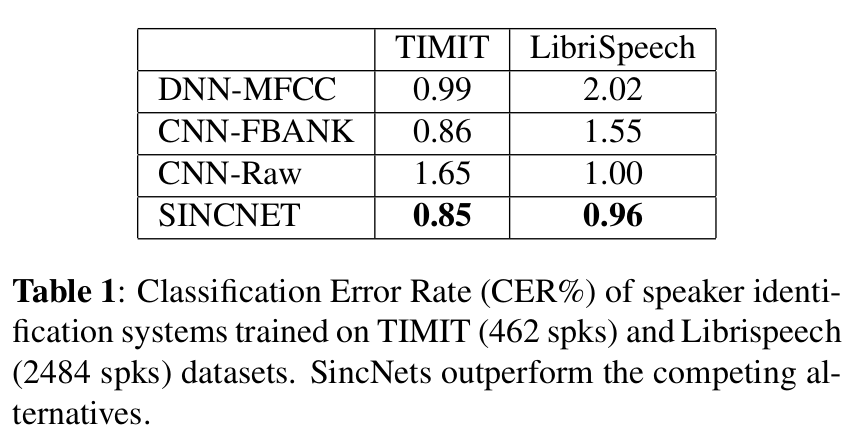
\includegraphics[width=.75\textwidth]{images/performance_speaker_identification.png}
		\caption{Bảng kết quả SicNet trong tác vụ nhận dạng giọng nói - SI}
		\label{fig:writing-thesis}
	\end{figure}
	Bảng trên đây là một bảng báo cáo về tỉ lệ phân lớp lỗi (\textbf{Classification Error Rates - CER\%}), khi thực nghiệm SincNet cùng với số kỹ thuật khác như \textbf{DNN-MFCC, CNN-FBANK, CNN-Raw} trên hai tập dữ liệu \textbf{TIMIT} và \textbf{LibriSpeech}. Nhìn chung, SincNet luôn dẫn đầu về độ lỗi tốt (có độ lỗi thấp nhất). Độ lỗi của \textbf{CNN-Raw} thật sự lớn khi tiến hành với tập TIMIT, điều này cho thấy S\textbf{SincNet} của chúng ta hoạt động tốt ngay cả khi có không lớn dữ liệu huấn luyện có sẵn. Khi huấn luyện với \textbf{LibriSpeech}, độ lỗi \textbf{CNN-Raw} giảm xuống, chúng ta có 4\% độ lỗi được giảm xuống, điều này cho thấy tốc độ hội tụ của SincNet cải thiện rõ ràng (1200 và 1800 epochs). Với \textbf{DNN-MFCC, CNN-FBANK}, hai kỹ thuật này hoạt động tốt trên \textbf{TIMIT} (vì đơn giản là \textbf{TIMIT} không lớn cho lắm như \textbf{LibriSpeech}), khi sang \textbf{LibriSpeech}, chúng có vẻ mất đi tính ổn định, độ lỗi cao lên.
	\textbf{Các kết quả đối với tác vụ xác minh người nói: } Thử nghiệm cuối cùng mà nhóm tác giả trình bày ở trong bài báo là tác vụ \textbf{xác minh giọng nói - Speaker Verification}. Bảng dưới đây, được trích ra trong bài báo, báo cáo về chỉ số \textbf{Equal Error Rate} (EER\%) khi thực nghiệm trên tập \textbf{LibriSpeech}. 
	\begin{figure}[H]
		\centering
		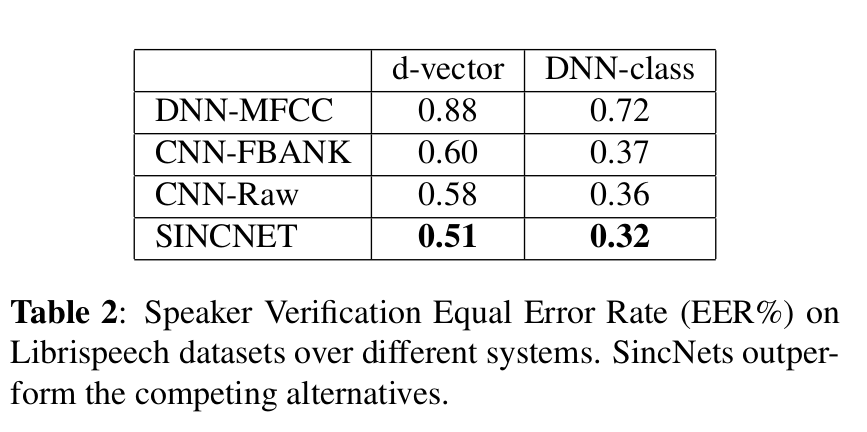
\includegraphics[width=.75\textwidth]{images/performance_speaker_verification.png}
		\caption{Bảng kết quả SicNet trong tác vụ xác minh giọng nói - SV}
		\label{fig:writing-thesis}
	\end{figure}
	
	Tất cả các mô hình DNN đều cho thấy hiệu suất đầy hứa hẹn, \textbf{các chỉ EER thấp hơn 1\% trong mọi trường hợp}. Bảng cũng cho thấy rằng \textbf{SincNet lại một lần nữa hoạt động tốt hơn các mô hình khác}, cho thấy sự cải thiện hiệu suất tương đối khoảng \textbf{11\% so với mô hình CNN}. Các mô hình lớp DNN hoạt động tốt hơn đáng kể so với các \textbf{d-vector}. Bất chấp hiệu quả của cách tiếp cận sau này, một mô hình DNN mới phải được huấn luyện (hoặc tinh chỉnh) cho mỗi người nói mới được thêm vào nhóm. Điều này làm cho cách tiếp cận này hoạt động tốt hơn, nhưng kém linh hoạt hơn so với \textbf{d-vector}.
	
	Để hoàn thiện hơn, nhóm tác giả cũng tiến hành các thí nghiệm khác với các \textbf{i-vector} tiêu chuẩn. Tuy nhiên so sánh chi tiết với kỹ thuật này nằm ngoài phạm vi của bài báo nên nhóm tác giả chỉ nêu ra những điểm đáng chú ý nhất trong kết quả. Hệ thống \textbf{i-vector} tốt nhất của nhóm tác giả đạt được \textbf{EER = 1,1\%}, \textbf{khá xa so với những gì đạt được với hệ thống DNN}. Tài liệu nổi tiếng rằng \textbf{i-vector} cung cấp hiệu suất cạnh tranh khi sử dụng nhiều dữ liệu huấn luyện hơn cho mỗi người nói và khi các câu kiểm tra dài hơn được sử dụng. Trong các điều kiện thách thức phải đối mặt trong công việc này, mạng neural đạt được khả năng tổng quát hóa tốt hơn.
	
	\textbf{Nhận xét về kiến trúc SincNet}
	\begin{itemize}
		\item Cơ sở lý thuyết Toán học vững vàng: Kỹ thuật band-pass filter, Window trong Xử lý tín hiệu số.
		\item Tính toán nhanh và gọn nhẹ: Như đã nói, đây là một đặc điểm của SincNet nhờ vào dùng ít tham số, kernel đối xứng.
		\item Kết hợp với Deep Learning một cách hiệu quả.
		\item Sử dùng DNN-Class trong đánh giá, cho kết quả đầy hứa hẹn, có độ lỗi EER thấp
	\end{itemize}
	Nhưng vẫn có hạn chế
	\begin{itemize}
		\item DNN-class tuy có EER thấp nhưng đánh đổi nhiều sự linh hoạt so với d-vectors
	\end{itemize}


	\section{E. Thực nghiệm của nhóm}
	\subsection{E.1 Phương pháp}
	Cài đặt mô hình Nhận dạng Người nói và đánh giá nó với tiếng Việt và tiếng Anh với SincNet.
	Các tác vụ thành phần của mô hình: Identification (Định danh) và Verification (Xác minh)
	
	\subsection{E.2 Kho ngữ liệu}
	\qquad \textbf{Tiếng Anh} Sử dụng hai tập dữ liệu đã được đề cập trong bài báo
	
	Với \textbf{TIMIT}, ta có một kho ngữ liệu với 462 người nói, các khoảng không phải lời nói ở đầu và cuối mỗi câu đã bị xóa, những tập tin về nội dung câu nói của TIMIT cũng được loại bỏ. Sau khi tinh chỉnh toàn bộ dữ liệu, tác giả dùng 5 câu nói của mỗi người nói để huấn luyện, 3 câu nói của mỗi người nói dùng để kiểm tra.
	
	Với tập ngữ liệu \textbf{LibriSpeech}, những phần với độ im lặng bên trong kéo dài hơn 125 ms được chia thành nhiều phần nhỏ. Việc chia tập huấn luyện (training set), tập kiểm tra (testing set) là ngẫu nhiên bằng cách chọn 12-15 giây dữ liệu huấn luyện của mỗi người nói và các câu kiểm tra kéo dài từ 2-6 giây. 
	
	\textbf{Tiếng Việt} Sử dụng tập dữ liệu Son et al. Dataset
	
	Nguồn dữ liệu từ bài báo Vietnamese Speaker Authentication Using Deep Models
	\begin{itemize}
		\item Dung lượng của tập dữ liệu: 535 MB
		\item Số mẫu trong tập dữ liệu: 400 mẫu
		\item Bộ dữ liệu gồm: hai tập  Men và Women, mỗi tập con chứa 10 thư mục người nói. Mỗi thư mục người nói chứa 20 đoạn ghi âm, chia ra Long và Short (mỗi loại 10 đoạn) 
		\item Nội dung câu nói
		\begin{itemize}
			\item Câu ngắn: “Tôi là sinh viên chuyên ngành công nghệ thông tin"
			\item Câu dài: "Tôi là sinh viên Học viện Công nghệ Bưu chính Viễn thông, chương trình đào tạo khá nặng đòi hỏi sinh viên phải học tập và nghiên cứu rất nhiều nhưng tôi tự hào vì đó là ngành đã và đang làm thay đổi cuộc sống xã hội loài người".
		\end{itemize}
		\item Điểm hạn chế: Bộ dữ liệu có kích thước khá nhỏ
	\end{itemize}
	
	Ngoài ra, nhóm tự ghi âm thêm dữ liệu với độ dài tương tự như tập này.
	\subsection{E.3 Thực nghiệm}
	\subsubsection{E.3.1 Thực nghiệm trên tập TIMIT}
	\begin{itemize}
		\item Xử lý dữ liệu
		\item Mô hình 
		\begin{itemize}
			\item Các cửa sổ có $\text{fs} = 16000$, tín hiệu được cắt thành những chunks với $\text{cw\_len}=200$, overlap $\text{cw\_shift}=10$s
			\item Lớp Input: sử dụng 80 bộ lọc SincNet có kích thước $L=251$, max pool - 3, sử dụng Layer Norm cho cả input và output, không dùng Batch Norm, hàm kích hoạt activation leaky-ReLU, dropout = 0
			\item Hai lớp CNN: sử dụng 2 lớp CNN, với mỗi lớp dùng 60 bộ lọc có kích thuốc $L=5$, sử dụng Layer Norm cho cả input và output, không dùng Batch Norm, hàm kích hoạt activation leaky-ReLU, dropout = 0
			\item Ba lớp DNN: sử dụng 3 lớp DNN (Multi Layer Perceptron) fully-connected với 2048 neurons, Layer Norm cho input, Batch Norm cho output, các lớp ẩn (hidden layers) dùng leaky-ReLU
			\item Lớp Output: Multi Layer Perceptron, 462 nodes, không dropout, không LayerNorm, không BatchNorm cho cả input và output, hàm activation function dùng softmax
			\item Hàm mất mát: Negative Log Likelihood Loss
		\end{itemize}
		\item Hyper parameters
		\begin{itemize}
			\item learning rate $\text{lr} = 0.001$
			\item $\alpha = 0.95$
			\item $\epsilon = 10^{-7}$
			\item $\text{batch\_size}=128$
			\item $\text{N\_epochs}=100$
			\item $\text{N\_batches}=800$
			\item $\text{N\_eval\_epoch}=8$
			\item $\text{seed}=1234$
		\end{itemize}
	\end{itemize}
	\subsubsection{E.3.2 Thực nghiệm trên tập Librispeech}
	\begin{itemize}
		\item Xử lý dữ liệu
		\item Mô hình 
		\begin{itemize}
			\item Các cửa sổ có $\text{fs} = 8000$, tín hiệu được cắt thành những chunks với $\text{cw\_len}=375$, overlap $\text{cw\_shift}=10$s
			\item Lớp Input: sử dụng 80 bộ lọc SincNet có kích thước $L=251$, max pool - 3, sử dụng Layer Norm cho cả input và output, không dùng Batch Norm, hàm kích hoạt activation leaky-ReLU, dropout = 0
			\item Hai lớp CNN: sử dụng 2 lớp CNN, với mỗi lớp dùng 60 bộ lọc có kích thuốc $L=5$, sử dụng Layer Norm cho cả input và output, không dùng Batch Norm, hàm kích hoạt activation leaky-ReLU, dropout = 0
			\item Hai lớp DNN: sử dụng 2 lớp DNN (Multi Layer Perceptron) fully-connected với 2048 neurons, Layer Norm cho input, Batch Norm cho output, các lớp ẩn (hidden layers) dùng leaky-ReLU làm activation cho lớp DNN thứ nhất, lớp kia dùng linear
			\item Lớp Output: 2 lớp Multi Layer Perceptron, 2048 nodes cho mỗi lớp, không dropout, Layer Norm cho input, Batch Norm cho output, hàm activation function lớp thứ nhất dùng leaky-ReLU, lớp thứ hai dùng softmax
			\item Hàm mất mát: Negative Log Likelihood Loss
		\end{itemize}
		\item Hyper parameters
		\begin{itemize}
			\item learning rate $\text{lr} = 0.001$
			\item $\alpha = 0.95$
			\item $\epsilon = 10^{-7}$
			\item $\text{batch\_size}=128$
			\item $\text{N\_epochs}=100$
			\item $\text{N\_batches}=100$
			\item $\text{N\_eval\_epoch}=10$
			\item $\text{reg\_factor}=1000$
			\item $\text{fact\_amp=0.2}$
			\item $\text{seed}=1234$
		\end{itemize}
	\end{itemize}
	\subsubsection{E.3.2 Thực nghiệm trên tập Son et al. Dataset}
	\begin{itemize}
		\item Xử lý dữ liệu
		\item Mô hình 
			\begin{itemize}
			\item Các cửa sổ có $\text{fs} = 16000$, tín hiệu được cắt thành những chunks với $\text{cw\_len}=200$, overlap $\text{cw\_shift}=10$s
			\item Lớp Input: sử dụng 80 bộ lọc SincNet có kích thước $L=251$, max pool - 3, sử dụng Layer Norm cho cả input và output, không dùng Batch Norm, hàm kích hoạt activation leaky-ReLU, dropout = 0
			\item Hai lớp CNN: sử dụng 2 lớp CNN, với mỗi lớp dùng 60 bộ lọc có kích thuốc $L=5$, sử dụng Layer Norm cho cả input và output, không dùng Batch Norm, hàm kích hoạt activation leaky-ReLU, dropout = 0
			\item Ba lớp DNN: sử dụng 3 lớp DNN (Multi Layer Perceptron) fully-connected với 2048 neurons, Layer Norm cho input, Batch Norm cho output, các lớp ẩn (hidden layers) dùng leaky-ReLU
			\item Lớp Output: Multi Layer Perceptron, 18 nodes, không dropout, không LayerNorm, không BatchNorm cho cả input và output, hàm activation function dùng softmax
			\item Hàm mất mát: Negative Log Likelihood Loss
		\end{itemize}
		\item Hyper parameters
		\begin{itemize}
			\item learning rate $\text{lr} = 0.001$
			\item $\alpha = 0.95$
			\item $\epsilon = 10^{-7}$
			\item $\text{batch\_size}=128$
			\item $\text{N\_epochs}=300$
			\item $\text{N\_batches}=100$
			\item $\text{N\_eval\_epoch}=1$
			\item $\text{seed}=1234$
		\end{itemize}
	\end{itemize}
	\subsection{E.4 Các kết quả}
	\subsubsection{E.4.1 Kết quả thực nghiệm trên tập TIMIT}
	\begin{figure}[H]
		\centering
		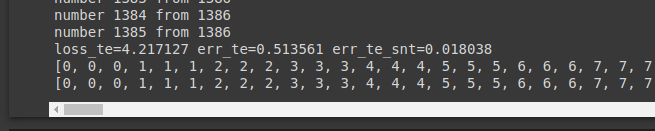
\includegraphics[width=.75\textwidth]{result/evaluate_result_timit.png}
		\caption{Kết quả thực nghiệm trên TIMIT Dataset}
		\label{fig:writing-thesis}
	\end{figure}
	\begin{figure}[H]
		\centering
		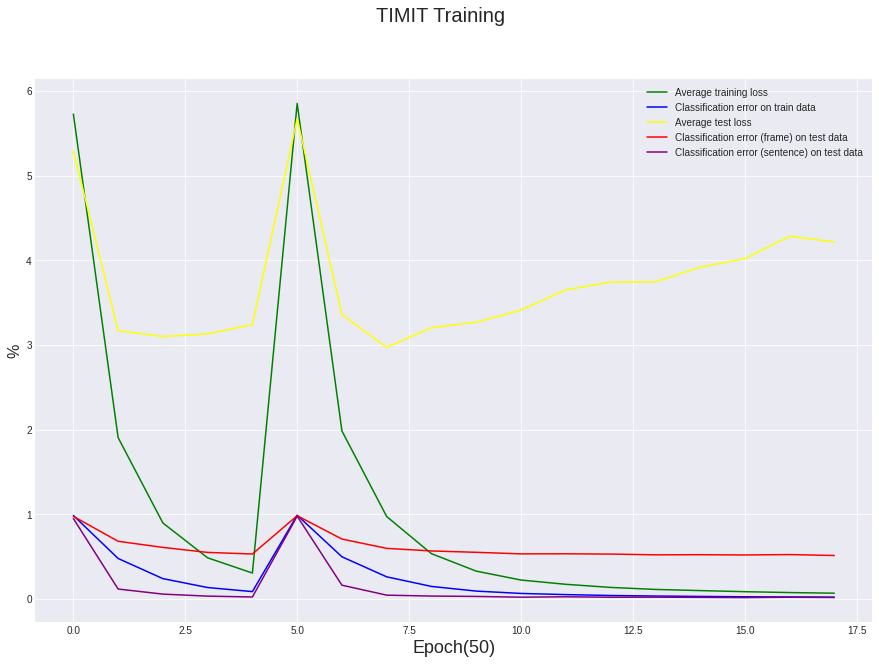
\includegraphics[width=.75\textwidth]{result/sincnet_timit_plot.png}
		\caption{Kết quả thực nghiệm trên TIMIT Dataset}
		\label{fig:writing-thesis}
	\end{figure}
	\subsubsection{E.4.2 Kết quả thực nghiệm trên tập Librispeech}
	\begin{figure}[H]
		\centering
		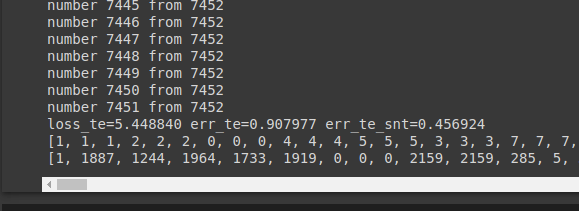
\includegraphics[width=.75\textwidth]{result/evaluate_result_libris.png}
		\caption{Kết quả thực nghiệm trên Librispeech Dataset}
		\label{fig:writing-thesis}
	\end{figure}
	\begin{figure}[H]
		\centering
		\includegraphics[width=.75\textwidth]{result/sincnet_librispeech_plot.png}
		\caption{Kết quả thực nghiệm trên Librispeech Dataset}
		\label{fig:writing-thesis}
	\end{figure}
	\subsubsection{E.4.3 Kết quả thực nghiệm trên tập Son et al. Dataset}
	\begin{figure}[H]
		\centering
		\includegraphics[width=.75\textwidth]{result/evaluate_result_vn_speaker.png}
		\caption{Kết quả thực nghiệm trên Son et al. Dataset}
		\label{fig:writing-thesis}
	\end{figure}
	\begin{figure}[H]
		\centering
		\includegraphics[width=.75\textwidth]{result/sincnet_vietnamese_plot.png}
		\caption{Kết quả thực nghiệm trên Son et al. Dataset}
		\label{fig:writing-thesis}
	\end{figure}
	\subsection{E.5 Những nhận xét}
	
	\nocite{*}
	\bibliography{references}\newpage\cleardoublepage
	\bibliographystyle{plain}
	
\end{document}
